% Template for PLoS
% Version 3.5 March 2018
%
% % % % % % % % % % % % % % % % % % % % % %
%
% -- IMPORTANT NOTE
%
% This template contains comments intended 
% to minimize problems and delays during our production 
% process. Please follow the template instructions
% whenever possible.
%
% % % % % % % % % % % % % % % % % % % % % % % 
%
% Once your paper is accepted for publication, 
% PLEASE REMOVE ALL TRACKED CHANGES in this file 
% and leave only the final text of your manuscript. 
% PLOS recommends the use of latexdiff to track changes during review, as this will help to maintain a clean tex file.
% Visit https://www.ctan.org/pkg/latexdiff?lang=en for info or contact us at latex@plos.org.
%
%
% There are no restrictions on package use within the LaTeX files except that 
% no packages listed in the template may be deleted.
%
% Please do not include colors or graphics in the text.
%
% The manuscript LaTeX source should be contained within a single file (do not use \input, \externaldocument, or similar commands).
%
% % % % % % % % % % % % % % % % % % % % % % %
%
% -- FIGURES AND TABLES
%
% Please include tables/figure captions directly after the paragraph where they are first cited in the text.
%
% DO NOT INCLUDE GRAPHICS IN YOUR MANUSCRIPT
% - Figures should be uploaded separately from your manuscript file. 
% - Figures generated using LaTeX should be extracted and removed from the PDF before submission. 
% - Figures containing multiple panels/subfigures must be combined into one image file before submission.
% For figure citations, please use "Fig" instead of "Figure".
% See http://journals.plos.org/plosone/s/figures for PLOS figure guidelines.
%
% Tables should be cell-based and may not contain:
% - spacing/line breaks within cells to alter layout or alignment
% - do not nest tabular environments (no tabular environments within tabular environments)
% - no graphics or colored text (cell background color/shading OK)
% See http://journals.plos.org/plosone/s/tables for table guidelines.
%
% For tables that exceed the width of the text column, use the adjustwidth environment as illustrated in the example table in text below.
%
% % % % % % % % % % % % % % % % % % % % % % % %
%
% -- EQUATIONS, MATH SYMBOLS, SUBSCRIPTS, AND SUPERSCRIPTS
%
% IMPORTANT
% Below are a few tips to help format your equations and other special characters according to our specifications. For more tips to help reduce the possibility of formatting errors during conversion, please see our LaTeX guidelines at http://journals.plos.org/plosone/s/latex
%
% For inline equations, please be sure to include all portions of an equation in the math environment.  For example, x$^2$ is incorrect; this should be formatted as $x^2$ (or $\mathrm{x}^2$ if the romanized font is desired).
%
% Do not include text that is not math in the math environment. For example, CO2 should be written as CO\textsubscript{2} instead of CO$_2$.
%
% Please add line breaks to long display equations when possible in order to fit size of the column. 
%
% For inline equations, please do not include punctuation (commas, etc) within the math environment unless this is part of the equation.
%
% When adding superscript or subscripts outside of brackets/braces, please group using {}.  For example, change "[U(D,E,\gamma)]^2" to "{[U(D,E,\gamma)]}^2". 
%
% Do not use \cal for caligraphic font.  Instead, use \mathcal{}
%
% % % % % % % % % % % % % % % % % % % % % % % % 
%
% Please contact latex@plos.org with any questions.
%
% % % % % % % % % % % % % % % % % % % % % % % %

\documentclass[10pt,letterpaper]{article}
\usepackage[top=0.85in,left=2.75in,footskip=0.75in]{geometry}

% amsmath and amssymb packages, useful for mathematical formulas and symbols
\usepackage{amsmath, amssymb, mathtools, amsthm}
% Use adjustwidth environment to exceed column width (see example table in text)
\usepackage{changepage}

% Use Unicode characters when possible
\usepackage[utf8x]{inputenc}

% textcomp package and marvosym package for additional characters
\usepackage{textcomp,marvosym}

% cite package, to clean up citations in the main text. Do not remove.
\usepackage{cite}

% Use nameref to cite supporting information files (see Supporting Information section for more info)
\usepackage{nameref,hyperref}

% line numbers
\usepackage[right]{lineno}

% ligatures disabled
\usepackage{microtype}
\DisableLigatures[f]{encoding = *, family = * }

% color can be used to apply background shading to table cells only
\usepackage[table]{xcolor}

% array package and thick rules for tables
\usepackage{array}

\usepackage{siunitx}
\usepackage{caption}
\usepackage{subcaption}

% create "+" rule type for thick vertical lines
\newcolumntype{+}{!{\vrule width 2pt}}

% create \thickcline for thick horizontal lines of variable length
\newlength\savedwidth
\newcommand\thickcline[1]{%
  \noalign{\global\savedwidth\arrayrulewidth\global\arrayrulewidth 2pt}%
  \cline{#1}%
  \noalign{\vskip\arrayrulewidth}%
  \noalign{\global\arrayrulewidth\savedwidth}%
}

% \thickhline command for thick horizontal lines that span the table
\newcommand\thickhline{\noalign{\global\savedwidth\arrayrulewidth\global\arrayrulewidth 2pt}%
\hline
\noalign{\global\arrayrulewidth\savedwidth}}


% Remove comment for double spacing
%\usepackage{setspace} 
%\doublespacing

% Text layout
\raggedright
\setlength{\parindent}{0.5cm}
\textwidth 5.25in 
\textheight 8.75in

% Bold the 'Figure #' in the caption and separate it from the title/caption with a period
% Captions will be left justified
\usepackage[aboveskip=1pt,labelfont=bf,labelsep=period,justification=raggedright,singlelinecheck=off]{caption}
\renewcommand{\figurename}{Fig}

% Use the PLoS provided BiBTeX style
\bibliographystyle{plos2015}

% Remove brackets from numbering in List of References
\makeatletter
\renewcommand{\@biblabel}[1]{\quad#1.}
\makeatother



% Header and Footer with logo
\usepackage{lastpage,fancyhdr,graphicx}
\usepackage{epstopdf}
%\pagestyle{myheadings}
\pagestyle{fancy}
\fancyhf{}
%\setlength{\headheight}{27.023pt}
%\lhead{\includegraphics[width=2.0in]{PLOS-submission.eps}}
\rfoot{\thepage/\pageref{LastPage}}
\renewcommand{\headrulewidth}{0pt}
\renewcommand{\footrule}{\hrule height 2pt \vspace{2mm}}
\fancyheadoffset[L]{2.25in}
\fancyfootoffset[L]{2.25in}
\lfoot{\today}

%% Include all macros below

\newcommand{\lorem}{{\bf LOREM}}
\newcommand{\ipsum}{{\bf IPSUM}}


\newcommand\restr[2]{{% we make the whole thing an ordinary symbol
\left.\kern-\nulldelimiterspace % automatically resize the bar with \right
#1 % the function
\vphantom{\big|} % pretend it's a little taller at normal size
\right|_{#2} % this is the delimiter
}}

\newcommand{\VV}[1]{\textcolor{red}{VV: #1}}
\newcommand{\AP}[1]{\textcolor{blue}{AP: #1}}
\newcommand{\JR}[1]{\textcolor{orange}{JR: #1}}
% \newcommand{\NS}[1]{\textcolor{orange}{Not sure: #1}}

\newcommand{\comment}[1]{}

\newcommand{\ie}{\emph{i.e.}\;}
\newcommand{\cfb}{\emph{cf.}\;}
\newcommand{\eg}{\emph{e.g.}\;}
\newcommand{\etal}{\emph{et al.}\;}

\newcommand{\partialt}[1]{\dfrac{\partial#1}{\partial t}}
\newcommand{\partialx}[1]{\dfrac{\partial#1}{\partial x}}
\newcommand{\partialxx}[1]{\dfrac{\partial^2 #1}{\partial x^2}}
\newcommand{\fpartial}[1]{\dfrac{\partial}{\partial #1}}

%%% new commands for variables
\renewcommand{\i}{^{(i)}}
\newcommand{\1}{^{(1)}}
\newcommand{\2}{^{(2)}}

\newcommand{\lip}{\mathrm{Lip}}
\newcommand{\sign}{\mathrm{sign}}
\newcommand{\ds}{\displaystyle}
\newcommand{\ddt}{\frac{\dx{}}{\dx{t}}}

\newcommand{\grad}{\nabla}
\renewcommand{\div}{\nabla\cdot}
\newcommand{\Lap}{\Delta}
\newcommand{\R}{\mathbb{R}}

\newcommand*{\dd}{\mathop{\kern0pt\mathrm{d}}\!{}}
\newcommand {\es}  {\varepsilon}
\pdfstringdefDisableCommands{\def\eqref#1{(\ref{#1})}}

\newcommand {\f}   {\frac}
\newcommand {\p}   {\partial}
\newcommand {\ov}  {\overline}
\newcommand {\undel}  {\underline}
\newcommand{\norm}[1]{\left\lVert#1\right\rVert}
\newcommand{\abs}[1]{\left\lvert#1\right\rvert}

\newcommand{\scal}[2]{\left(#1 , #2\right)}
\newcommand{\lscal}[2]{\left(#1 , #2\right)^h}

\newcommand {\dt}   {\Delta t}
\newcommand {\x}   {\mathbf{x}}
\newcommand {\vel}   {\mathbf{v}}
\newcommand{\dx}{\, \mathrm{d}x}
\newcommand{\pdi}[2]{\frac{\partial #1}{\partial #2}}

\newcommand{\Cinulin}{$\prescript{14}{}{\text{C}}$-inulin }


\newtheorem{theorem}{Theorem}%[section]
\newtheorem{lemma}[theorem]{Lemma}
\newtheorem{definition}[theorem]{Definition}
\newtheorem{remark}[theorem]{Remark}
\newtheorem{proposition}[theorem]{Proposition}
\newtheorem{corollary}[theorem]{Corollary}


%% END MACROS SECTION


\begin{document}
\vspace*{0.2in}

% Title must be 250 characters or less.
\begin{flushleft}
{\Large
\textbf\newline{Multi-compartmental model of glymphatic clearance of solutes in brain tissue} % Please use "sentence case" for title and headings (capitalize only the first word in a title (or heading), the first word in a subtitle (or subheading), and any proper nouns).
}
\newline
% Insert author names, affiliations and corresponding author email (do not include titles, positions, or degrees).
\\
Alexandre Poulain\textsuperscript{1*},
Jørgen Riseth \textsuperscript{1},
Vegard Vinje\textsuperscript{1},
\\
\bigskip
\textbf{1} Department for Numerical Analysis and Scientific Computing, Simula Research Laboratory, Oslo, Norway
\\
\bigskip

% Insert additional author notes using the symbols described below. Insert symbol callouts after author names as necessary.
% 
% Remove or comment out the author notes below if they aren't used.
%
% Primary Equal Contribution Note
%\Yinyang These authors contributed equally to this work.

% Additional Equal Contribution Note
% Also use this double-dagger symbol for special authorship notes, such as senior authorship.
%\ddag These authors also contributed equally to this work.

% Current address notes
%\textcurrency Current Address: Dept/Program/Center, Institution Name, City, State, Country % change symbol to "\textcurrency a" if more than one current address note
% \textcurrency b Insert second current address 
% \textcurrency c Insert third current address

% Deceased author note
%\dag Deceased

% Group/Consortium Author Note
%\textpilcrow Membership list can be found in the Acknowledgments section.

% Use the asterisk to denote corresponding authorship and provide email address in note below.
* Corresponding author: poulain@simula.no

\end{flushleft}
% Please keep the abstract below 300 words
\section*{Abstract}
The Glymphatic system is the subject of numerous pieces of research in Biology. Mathematical modeling plays a considerable role in this field since it can indicate the possible physical effects in this system and validate the biologists' hypotheses. The available mathematical models that describe the system at the scale of the brain (\ie the macroscopic scale) are based solely on the diffusion equation and do not consider the fine structures formed by the perivascular spaces.   
 We propose a mathematical model representing the time and space evolution of a mixture flowing through multiple compartments to solve this issue. We adopt a macroscopic point of view in which the compartments are all present at the same point in space. The equations system is composed of two coupled equations for each compartment: one equation for the pressure of the cerebro-spinal fluid and one for the mass concentration of a molecule. The fluid and solute can move from one compartment to another according to certain membrane conditions modeled by transfer functions. We propose to apply this new modeling framework to the clearance of the molecule \Cinulin from the rat brain. 
 
% Please keep the Author Summary between 150 and 200 words
% Use first person. PLOS ONE authors please skip this step. 
% Author Summary not valid for PLOS ONE submissions.   
%\section*{Author summary}
%Lorem ipsum dolor sit amet, consectetur adipiscing elit. Curabitur eget porta erat. Morbi consectetur est vel gravida pretium. Suspendisse ut dui eu ante cursus gravida non sed sem. Nullam sapien tellus, commodo id velit id, eleifend volutpat quam. Phasellus mauris velit, dapibus finibus elementum vel, pulvinar non tellus. Nunc pellentesque pretium diam, quis maximus dolor faucibus id. Nunc convallis sodales ante, ut ullamcorper est egestas vitae. Nam sit amet enim ultrices, ultrices elit pulvinar, volutpat risus.

\linenumbers

% Use "Eq" instead of "Equation" for equation citations.
\section*{Introduction}
L% General presentation of the Glymphatic system
The proposed glymphatic system~\cite{Iliff_2012_PVS} explains clearance of metabolic waste from the brain and has been the subject of many pieces of research in the past decade~\cite{Holter9894,abbott_role_2018,jessen_glymphatic_2015}.
 This concept suggests that clearance of metabolic solutes in the brain is facilitated by specific pathways for exchange between interstitial fluid (ISF) and cerebrospinal fluid (CSF). This exchange occurs via perivascular spaces (PVSs), small fluid filled spaces surrounding blood vessels. 
According to the glymphatic theory, CSF enters the parenchyma via periarterial spaces and exits it via perivenous spaces. Furthermore, Iliff \etal~\cite{Iliff_2012_PVS} put forward that it exists a bulk flow of fluid in the interstitial space originating from the peri-arterial spaces and draining the metabolic waste toward the peri-venous spaces.  
Understanding the Glymphatic system is critically important since its impairment seems to be linked to serious issues such as Alzheimer's decease~\cite{reeves_glymphatic_2020}.

Even after a decade of research to verify this theory, many gray areas subsist. Indeed, some questions remain still to be answered: 
\textit{i)} Does the circulation of CSF as described by Iliff \etal~\cite{Iliff_2012_PVS} (inflow around arteries and outflow around veins) really occur? 
\textit{ii)} What are the mechanisms explaining the movement of CSF in the perivascular spaces?
\textit{iii)} Does convection in the interstitial space occur and is this flow sufficient to dominate transport? 

%Many biological experiments have been conducted to study these questions, we here cover only a few of them. The interested reader can find many references in the recent reviews~\cite{Holter9894,abbott_role_2018,jessen_glymphatic_2015}. 



% movement of CSF in PVS
In vivo studies using two-photon microscopy have imaged flow along periarterial spaces in the same direction as blood~\cite{bedussi-2018-paravascular,mestre_flow_2018}, suggesting these spaces act as a entry to the brain even though this claim is still debated~\cite{bakker2019paravascular}. 
%Furthermore, the two previously cited works indicate that this movement seems to be linked to cardiac cycle as it is pulsating and follows the direction of the blood flow. However, mathematical modellings of fluid movement in the CSF suggest that it is unlikely the case. Indeed, Daversin-Catty \etal~\cite{daversin-catty_mechanisms_2020} show using numerical simulations of CSF flow in a realistic PVS geometry that without a static CSF pressure gradient, whose origin remains to determine, PVS flow is not comparable to experimental findings. 

% movement in interstitial space and clearance
The question of the existence of a bulk flow of fluid in the interstitial space as proposed by Iliff \etal~\cite{Iliff_2012_PVS} remains open. Indeed, some pieces of research indicate that solute transport in the interstitial space is dominated by diffusion~\cite{asgari_glymphatic_2016, Holter9894, smith2019going}, while others claim that diffusion alone can not explain the transport of tracer from the brain~\cite{valnes_apparent_2020, ray2021quantitative}. In a recent study Ray \etal~\cite{ray_analysis_2019} concluded that transport of large molecules will be dominated by convection given expected ECS flow rates as reported in the literature. Convection-diffusion equations have been used to study this effect at the scale of the brain~\cite{ray_analysis_2019,valnes_apparent_2020,Holter9894,nicholson-1981-ion, stoverud_modeling_2012, ray2021quantitative, croci2019uncertainty}. These works helped gain some insights of the relevant mechanisms that may play a role for clearance of interstitial solutes. Their main conclusion is that it is unlikely that clearance is explained solely by diffusion within the parenchyma.   

Current mathematical models of glymphatic transport at the scale of the brain are limited to the convection-diffusion equation. In that case, the fluid velocities and concentrations are averaged between ECS and PVS (and all other routes of transport) to capture the overall spread of solutes. To this end multiple-compartment models that can distinguish between different compartments such as blood vessels and tissue have been used to study for example drug transport to the lung~\cite{Erbertseder-2012-lung} or clot fragmentation~\cite{Payne-clot-2021} with great detail. However, these models require detailed information on vessel structure and require too many degrees of freedom to study the brain at the macroscale. 

To solve these issues, homogenized models seem to be a good solution. Even though homogenization is often used for infiltration in porous media~\cite{Hornung-1996-homogenization}, such framework has been successfully applied to represent transport of solute and fluid in the interstitium and vascular network of vascularized tumors~\cite{ shipley_multiscale_2010,shipley-four-comp, Penta-homogenization-2015}.   
Furthermore, there is a connection between these models for biological applications and models for fluid movement in porous media. These models denominated by the acronym MPET (for \textit{Multiple-network poroelastic theory }), comprise the movement of fluid through multiple compartments that are embedded in an elastic medium~\cite{Biot-1941-Consolidation,Biot-1955-Consolidation2, Bai-MPET-1993,tully_ventikos_2011,Vardakis-2016-cerebral,Guo-2018-MPET,Guo-2019-MPET}.




%\paragraph{Content of the article.}
In this paper, we use a homogenized model to describe the glymphatic system and the blood perfusion at the scale of the brain. To validate the relevancy of our modelling framework, we study the clearance of the important molecule \Cinulin from the murine brain. 
More precisely, we propose a new multi-compartment model to represent the movement of the cerebro-spinal fluid through the different structures that are the subarachnoid space, the perivascular spaces, the interstitial space and the blood vascular tree. This modeling of the fluid's movement is coupled to diffusion-convection equations for each compartment to represent the clearance of one solute in the brain. 
We denominate our model the \textit{MPT model} (for \textit{Multiple-Porosity Theory}). 
Even though the model is general enough the consider different types of mechanisms (\ie convection, diffusion, membrane conditions), it retains information at the microscopic scale and allows for different properties in each compartment. %The equations system can be obtained from homogenization of a microscopic description of the Glymphatic system and assuming a periodic distribution of vessel throughout the brain or, in a simpler manner, from a continuum approach. 
%The model derivation presented in this article follows the second method.
To access the relevancy of such modelling framework, we compare the results obtained with the standard convection-diffusion equation (within one compartment) to our multi-compartment model for the representation of solute clearance in the murine brain. In particular, we consider two specific test cases for the molecule \Cinulin. This molecule is known to not cross the Blood-Brain Barrier (BBB in short). The two test cases allow to assess the importance of considering the blood perfusion in the system. To model these effects, we consider the applications represented in the two figures
Fig~\ref{fig:Cinulin-sketch} and Fig~\ref{fig:Cinulin-sketch7comps}.

\begin{figure}
\centering
\begin{subfigure}{.5\textwidth}
  \centering
  \caption{Clearance routes of \Cinulin.}
  \label{fig:Cinulin-sketch}
\end{subfigure}%
\begin{subfigure}{.5\textwidth}
  \centering
  \caption{Clearance routes of \Cinulin  through Glymphatic system and blood network.}
  \label{fig:Cinulin-sketch7comps}
\end{subfigure}
\caption{Illustrative representation of the different compartments for the MPT model for the modeling of \Cinulin clearance. Convective exchange of solute through the different compartments is indicated by red arrows while diffusive exchange by green ones.}
\label{fig:multi-comp}
\end{figure}






In Section~\ref{sec:method}, we present and motivate the mathematical models that we use. We introduce the initial and boundary conditions, carefully chosen to approximate the biological experiments. This section contains also the parameters' definitions and values for the two important molecules: Amyloid-$\beta$ and \Cinulin.
Section~\ref{sec:results} presents the numerical results and compares the simulation results with biological data. 
In Section~\ref{sec:discussion}, we use this section to discuss the relevancy of the mathematical models as well as its advantages compared to other models from the literature.      

This work is the first step toward bridging the gap between microscopic properties of the Glymphatic system and an efficient macroscopic modelling of fluid and solute transport within the brain. 


\section{Methods}
\label{sec:method}
\subsection{Mathematical models}
\paragraph{Notations.} We first specify some important notations that we use in the following of this article. We denote by $\Omega \subset \R^3$ the spatial domain, \ie the murine brain. We assume that the boundary of this domain $\p \Omega$ is sufficiently smooth. Therefore, we denote by $\x \in \Omega$, any point of this domain such that the coordinates are given by $\x =(x_1,x_2,x_3)$. We emphasize that, in the rest of this article, to denote vectors, we use bold symbols. Since we model the time evolution of the Glymphatic system, our time-space domain is denoted by $\Omega_T = \Omega \times [0,T]$, with $T> 0$ a finite time. We use two different mathematical models: the convection-diffusion model in a single compartment and a multicompartment model for fluid and solute transport. We use the following notation convention: when an unknown or a parameter is indicated with a subscript, it denotes its compartment. The subscript $j=e$ denotes the extracellular space and is used for both the multi-compartment model and the single compartment diffusion-convection equation. The subscripts $j=a$ and $j=pa$ denote respectively the arterial blood compartment and the periarterial compartment. The same is adopted for the venous and peri-venous compartments with the subscripts $j=v$ and $j=pv$. The capillary blood compartment is indicated by the subscript $j=c$ and $j=pc$ denotes the PVS compartment around capillaries.

\paragraph{The diffusion equation.}
To model the clearance of an interstitial solute in the murine brain, one of the simplest mathematical model to use is the diffusion equation. Denoting by $c_e = c_e(t,\x)$ the solute concentration in the extra-cellular space (\ie the interstitial space), the model reads
\begin{equation}
    \f{\p c_e}{\p t} = D_e^* \Delta c_e , \quad \forall \x\in \Omega,\quad t\in (0,T].
    \label{eq:diffusion-convection}
\end{equation}
In the previous model, $D_e^*$ is the effective diffusion coefficient of the molecule in the ECS.


\paragraph{The multicompartment model.}
To take into account the different structures in which the fluid flows, we consider the multiple compartments as depicted in the schematic illustrations given in Fig~\ref{fig:multi-comp}. Therefore, we denote by $J$ the set of compartments (\eg the set corresponding to Fig~\ref{fig:Cinulin-sketch} is $J={pa,e,pv}$) and we denote the pressure in the $j-$th compartment by $p_j = p_j(t,\x)$ and for the solute concentration $c_j = c_j(t,\x)$. 
The following model is denominated the MPT equation (in reference to the MPET equations~\cite{Bai_1993_Multiporosity, tully_ventikos_2011}, but in our case we do not consider displacement of the brain tissue).
We denote by $\phi_j$ denotes the porosity of the $j-$th compartment (\ie the relative volume taken by the pores of this compartment).
We emphasize that the compartments are all present at any point $\x\in \Omega$. Thus, under the assumption of incompressible flow, for all $\x\in \Omega,\, t\in (0,T]$, we have the equations' systems, for each $j\in J$
\begin{equation}
    \begin{cases}
         -  \nabla\cdot( \frac{\kappa_j}{\phi_j \mu_j} \nabla p_j) = r_j,\\ %\gamma_{j , i} \left[(p_i - p_j)-\sigma (\pi_i-\pi_j)\right],\\
          \begin{multlined} \frac{\partial c_j}{\partial t} - \frac{ \kappa_j}{\phi_j \mu_j}\div\left( p_j  \nabla c_j\right)  - D_j^* \Lap c_j 
         = s_j,
         \end{multlined}
    \end{cases}
    \label{eq:main-system}
\end{equation}
in which $\kappa_j$ is the permeability coefficient for the fluid in the interstitial space, $\mu_j$ is the dynamic viscosity of the fluid, $D_j^*$ is the effective diffusion coefficient in the $j$-th compartment, and $r_{j}, s_{j}$ are the transfer functions to model the exchanges between the compartments and will be described in the next paragraph. For details on the formal derivation of these equations, we refer the reader to the Appendix~\ref{app:derivation}. 
\paragraph{Transfer functions. }
The transfer functions in System~\eqref{eq:main-system} model the exchanges of fluid and solute through the different compartments. 
These compartments are separated by a membrane or are in communication between vessels (\eg an artery branching to capillaries or the PVS around arteries branching to the PVS around capillaries).

When the compartments are separated by a membrane, the fluid flows from one compartment to another due to a difference of pressure and the hydraulic conductivity of the membrane, \ie 
\begin{equation}
    r_j = \frac{1}{\phi_j}\sum_{i\in J, i\neq j} \gamma_{j , i} \left[(p_i - p_j)-\sigma_{ij}(\pi_i-\pi_j)\right],
\end{equation} 
with 
\begin{equation}
\gamma_{j , i} = L_{ij} \f{\abs{S_{ij}}}{\abs{\Omega}},
\end{equation}
where $L_{ij}$ is the hydraulic conductivity of the membrane separating the $i-$th and $j-$th compartments, $\f{\abs{S_{ij}}}{\abs{\Omega}}$ is the ratio between the surface of the membrane to the total volume of the tissue, and $\sigma_{ij}$ is the osmotic reflection coefficient for the membrane. This reflection coefficient corresponds to a specific solute. In this work, we only consider osmotic effects due to plasma cells in the blood. 
The solute crosses the membrane due to the combination of two effects: it is convected by the fluid through the pores of the membrane and it also diffuses. These two effects are depicted by the transfer functions
\begin{equation}
   %s_j = \frac{1}{\phi_j}  \sum_{i\in J, i\neq j}\lambda_{j , i} ( c_i- c_j) +  c_j \tilde \gamma_{j , i} \min(0,(p_i - p_j)-\sigma_{ij}(\pi_i-\pi_j)) +  c_i \tilde \gamma_{j , i} \max(0,(p_i - p_j)-\sigma_{ij}(\pi_i-\pi_j)),
    s_j = \frac{1}{\phi_j}  \sum_{i\in J, i\neq j}\lambda_{j , i} ( c_i- c_j) +  \frac{(c_j+c_i)}{2} \tilde \gamma_{j , i} (p_i - p_j-\sigma_{ij}(\pi_i-\pi_j)) ,
\end{equation}
where this time 
\[
    \lambda_{j , i} = P_{ij} \f{\abs{S_{ij}}}{\abs{\Omega}}, \quad \tilde \gamma_{j , i} =  \gamma_{j , i} (1-\sigma_\text{reflect}),
\]
in which $P_{ij}$ is the permeability of the membrane separating the $i-$th and $j-$th compartments to the solute and $\sigma_\text{reflect}$ again reflects the solvent-drag reflection coefficient. 


In the case of vessels branching to another type, no membrane is present. The exchange function reflects the free communication in these vessels and is defined differently. We provide in Subsection~\ref{subsec:para-values} values for the exchange coefficients $\gamma_{j , i}, \tilde \gamma_{j , i}, \lambda_{j , i}$ when they model branching of vessels or PVSs.   



%\VV{1) Diffusion convection equation. 2) Multiple compartment diffusion convection. 3) Velocities in 2) will come from MPT (list equations). }

\subsection{Description of the application}
We now describe the modeling of clearance of \Cinulin using Equation~\eqref{eq:diffusion-convection} and/or System~\eqref{eq:main-system}. 
This molecule is of interest because it is known to not cross the BBB and, hence, is cleared from another pathway. 

\paragraph{Clearance of \Cinulin}
To study the clearance of \Cinulin from the rat brain, we consider two modeling frameworks. 
%Since \Cinulin is not able to cross the blood-brain-barrier, molecules injected into the brain parenchyma will be confined to the ECS compartment.
It is not clear if \Cinulin injected into the frontal cortex of rats is confined in the interstitial space and is cleared from this compartment. Recent evidences show that depending on whether the animal is asleep or awake, difference in the speed of clearance are observed~\cite{Xie_2013_sleep}. To investigate a possible enhancement of the clearance of \Cinulin due to the Glymphatic system, we consider two applications of our mathematical models.

We first assume that bulk flow of fluid in the interstitial space is negligible and clearance occurs due to diffusion in the interstitial space only. Hence, we use Equation~\eqref{eq:diffusion-convection} with $\vel_e = 0$. Clearance of \Cinulin occurs at the brain surface and is modelled by appropriate boundary conditions that are described below. 

Secondly, we consider a clearance of \Cinulin due to the Glymphatic system. Hence, we use System~\eqref{eq:main-system} with $\abs{J}=4$ compartments: ECS, PVS around arteries, PVS around capillaries, and PVS around veins. Fig~\ref{fig:Cinulin-sketch} depicts this scenario. CSF is assumed to flow from the PVS around arteries to the PVS around capillaries or in the interstitial space. From the PVS around capillaries, CSF flows in the interstitial space or in the PVS around veins. From the interstitial space CSF is reabsorbed in the PVS around veins or capillaries. Clearance from the brain occurs at the brain surface from the interstitial space or the PVS around veins, or eventually arteries.
In the following, we denote the extracellular space by the index $j=e$, the PVS around arteries by $j=pa$, around capillaries by $j=pc$, and around veins by $j=pv$. 

For the sake of clarity, in the following we refer to these applications of our modeling framework as
\begin{itemize}
    \item \textbf{\Cinulin test case 1:} Diffusion only in the interstitial space modeled by Equation~\eqref{eq:diffusion-convection} with $\vel_e = 0$. 
    \item \textbf{\Cinulin test case 2:} Clearance from the Glymphatic system using System~\eqref{eq:main-system} with $J=4$ compartments. 
    \item \textbf{\Cinulin test case 2:} Clearance from the Glymphatic system and considering the blood network using System~\eqref{eq:main-system} with $J=7$ compartments. 
\end{itemize}



\subsection{Initial and boundary conditions} \label{subsec:Init-bound}
\paragraph{Initial condition}

We consider the application in which the solute is injected directly into the rat cortex, and assume that the initial \Cinulin concentration is given as a three-dimensional Gaussian around the center of injection $ \mathbf{s} $,
\begin{equation}
    c_e(0, \x) = C^0 \exp{\frac{|\x - \mathbf{s}|^2}{\sigma^2}} 
    \label{eq:inulin-initial}
\end{equation}
where $C^0$ is a reference concentration, and $ \sigma $ determines the initial spread of the solute after injection. The reference concentration is chosen such that the integral of the initial condition over the domain matches the injected tracer amount. We emphasize that the initial condition is the same for the case of one compartment and when multiple compartments are considered.  
%See figure \tempref{inulin diffusion} for a visualization.

%\subparagraph{Amyloid-$\beta$}
%When the convection-diffusion is used, the initial condition is the same as for \Cinulin and is given by Equation~\eqref{eq:inulin-initial}. 
%However, for the multi-compartment model, the initial point of injection is assumed to be in the interstitial space, \ie
%\begin{equation}
%    c_e(0,\x) = C^0 \exp{\frac{|\x - \mathbf{s}|^2}{\sigma^2}}, \quad \text{and} \quad c_j(0,\x) = 0,\quad \text{for}\quad j\in J, j\neq e, 
%    \label{eq:amyloid-initial-mc}
%\end{equation}
%where $\mathbf{s}$ is the center of injection.


\paragraph{Boundary conditions}
We describe the boundary conditions for the multicompartment model. The boundary conditions for the diffusion model are simply given assuming that the extracellular space is the only compartment and that $\mathbf{v}_e = 0$.

We start by giving the boundary conditions for the pressure equations. 
To generate a relevant bulk flow within the PVSs, we assume a slight pressure difference between the boundary of the PVSs around arteries and veins.
We know that intracranial pressure in murine is $4 \pm 0.74 \si{mmHg}$ (see~\cite{Roy-rat-pressure-2013}). 
Interstitial fluid pressure has been measured in murine~\cite{Wiig-1983-interstitial} and is $3.43 \pm 0.65  \si{mmHg}$.


Therefore, we choose for the modelling of the clearance of \Cinulin from the Glymphatic system corresponding to Fig~\ref{fig:Cinulin-sketch}
\begin{equation}
\begin{cases}
    - \frac{\kappa_e}{\mu_\text{CSF}}\frac{\partial p_e}{\partial \pmb{\nu}}(t,\mathbf{x}) = \gamma_{e , SAS}(p_\text{SAS}-p_{e}),\quad -\frac{\kappa_{pa}}{\mu_\text{CSF}}\frac{\partial p_{pa}}{\partial \pmb{ \nu}}(t,\mathbf x)  = \gamma_{\text{PVSpial},pa}(p_{\text{PVSpial}}-p_{pa}), \\
    \frac{\partial p_{pc}}{\partial \pmb{\nu}}(t,\mathbf x) = 0, \quad p_{pv} = 3.36\, \si{mmHg},  %-\frac{\kappa_{pv}}{\mu_{pv}} \frac{ \partial p_{pv}}{\partial \nu}(t,\mathbf x) = \gamma_{CSF , pv}(p_{v} - p_{pv}) , 
\end{cases}
\label{eq:BC-4compsPVS}
\end{equation}
$\text{on } \partial \Omega,\, t>0$, with $\pmb{\nu}$ being the outward normal vector to the boundary $\partial \Omega$ and $p_\text{PVSpial} = 4.74\si{mmHg} $ is the CSF pressure inside the PVS of pial arteries and $p_\text{SAS} = 3.74 \si{mmHg} $ is the CSF pressure inside the subarachnoid space. The coefficients $\gamma_{\text{PVSpial},pa}, \gamma_{SAS , e}$ are related to the permeability of the pial surface of the brain for the CSF.
%The difference of applied pressure between the different PVS compartments is explained by our aim to produce a bulk flow that represents the Glymphatic system , \ie inflow around arteries and outflow around veins.

For the blood flow (see Fig~\ref{fig:Cinulin-sketch7comps}) we also need the boundary conditions
\begin{equation}
\begin{cases}
    -\frac{\kappa_{a}}{\mu_{a}}\frac{\partial p_{a}}{\partial \pmb{\nu}}(t,\mathbf x)  = \frac{B_\text{blood}}{A_\text{brain}}, \\
    \frac{\partial p_{c}}{\partial \pmb{\nu}}(t,\mathbf x) = 0, \quad p_{v}(t,\mathbf x) = 7.0\, \si{mmHg}, 
\end{cases}
\text{ on } \partial \Omega, \, t>0,
    \label{eq:BC-4compsblood}
\end{equation}
for which $\frac{B_\text{blood}}{A_\text{brain}} $ is a specified inflow ($B_\text{blood}=100\, \si{mL/100g/min} \times \text{mass}_\text{brain} = 33.33 \,\si{mm^3/s}$). 
The previous values are found using the measurements from~\cite{mayhan_role_1986}.


For the concentration equations, different boundary conditions are considered. 
Indeed, the first and simplest approach is to use homogeneous Dirichlet boundary conditions to represent clearance from the tissue and zero-flux boundary conditions for the compartments that are not in communication with the subarachnoid space. Namely, we impose Dirichlet boundary conditions for the concentration equations in the venous, arterial, peri-arterial, peri-venous and extracellular spaces since these compartments represent possible outflow routes. For the other compartments we assume that there is no flow at the surface of the brain. Thus, we have
\begin{equation*}
    \begin{cases}
    c_j \big|_{\partial \Omega} =  0 ,\quad \text{for}\quad j=\{a,v,pa,pv,e \}, \\
    \frac{\partial\left( D_j \nabla c_j + \frac{\kappa_j}{\mu_j}c_j \nabla p_j\right)}{\partial \nu}  = 0\quad \text{on } \partial \Omega, \text{ and for } j = \{c,pc\}.
    \end{cases}
\end{equation*}
In practice, this condition assumes that \Cinulin in the ECS at the cortical surface is instantly absorbed in the CSF. Moreover, it requires that the clearance of solute from the subarachnoid space is sufficiently quick, so that the \Cinulin concentration in the CSF is negligible. 

To represent the concentration of solute within the CSF in the subarachnoid space, we modify the Dirichlet boundary conditions to
\begin{equation}
     \restr{c_j}{\partial \Omega} =  g(t),\quad \text{for}\quad j=\{a,v,pa,pv,e \}, \quad t >0,
    \label{eq:inulin-inhomogeneous-dirichlet}
\end{equation}
where $ g $ is given as the total amount of molecules that has been cleared from the brain up to that time, averaged over the CSF volume $ V_\text{CSF} $ in the fluid filled space surrounding the brain, \ie the subarachnoid space. The rate of change of molecules tracer within the parenchyma, per unit of time, is given by
\begin{equation}
    \frac{d}{dt}\int_{\Omega} \sum_{j\in J} \phi_j c_j \,\dd \x= \sum_{j\in J} \int_{\Omega} \phi_j \frac{\partial c_j}{\partial t} \,\dd \x=   - \int_{\partial \Omega}  \mathbf{q} \cdot \pmb{\nu} \,\dd s  ,
\end{equation}
in which $\mathbf{q}$ is the mass total flux from all the compartments at the surface of the brain (we recall that $\pmb{\nu}$ is the outward pointing normal to the surface of the brain). 
For each compartment this flux is given by the combination of diffusion and convection 
\[
    \mathbf{q} =  \sum_{j\in J}  - D_j\nabla c_j + c_j \mathbf{v}_j,\quad \mathbf{v}_j = -\frac{\kappa_j}{\mu_j}\nabla p_j.   
\]
A decrease of molecules within the brain, corresponds to an increase of concentration in the subarachnoid space, and vice-versa. Therefore, $g$ is solution of the linear ordinary differential equation 
\begin{equation}
    \begin{cases}
        \frac{dg}{dt} &= - \alpha g(t)  + \frac{1}{V_\text{CSF}} \int_{\partial \Omega}  \mathbf{q} \cdot\pmb{\nu}\,\dd s,\\
        g(0) &= 0,
    \end{cases}
    \label{eq:inulin-boundary-inhomogeneous}
\end{equation}
where $\alpha > 0$ is the rate of clearance of CSF from the subarachnoid space. 
In practice, this model assumes instantaneous absorption of molecules in the CSF, and instant mixing of the solute within the whole subarachnoid space. Assuming that the diffusion coefficient in the CSF is much larger than within the ECS, then this model offers rough approximation for clearance, without significantly increasing the model complexity.

The latter Dirichlet boundary condition may be interpreted as a model for conservation of the amount of molecules if $\alpha =0$. Assuming that the molecules are not eliminated from the CSF, an alternate formulation of this condition is given by
\begin{equation}
    \sum_{j\in J} \int_\Omega  \phi_j c_j \,\dd x + g(t) V_{\text{CSF}} = N_0,
    \label{eq:inulin-tracer-conservation}
\end{equation}
where $N_0 = \sum_{j\in J} \int_\Omega  \phi_j c_j(0,\x) \,\dd x $ is the total amount of molecules injected into the brain. Thus, this time $g$ is simply given by 
\begin{equation}
    g(t) = \frac{1}{ V_{\text{CSF}}}\left( N_0  - \sum_{j\in J} \int_\Omega  \phi_j c_j \,\dd \x \right) .
    \label{eq:g-conservation}
\end{equation}



%The boundary conditions for the compartments $j \in \{e,pa,pc,pv\}$ is then given by Equation~\eqref{eq:inulin-boundary-inhomogeneous}.
%\begin{remark}
%We do no consider time dependent Dirichlet boundary conditions for the multicompartment model since, as shown by our numerical results in Section~\ref{sec:results}, the type of boundary conditions does not play a big role for the time scale considered in our study. 
%\end{remark}
%The interstitial space and perivascular spaces are in communication with the subarachnoid space. Therefore, as in the previous description of the boundary conditions for\Cinulin, we need to compute the concentration within the CSF in the subarachnoid space.


\subsection{Parameter values}
\label{subsec:para-values}

\subsubsection{For the convection-diffusion equation}

\paragraph{\Cinulin diffusion coefficient}
The free diffusion coefficient for \Cinulin is $ D_\text{free}^\text{\Cinulin} = 2.98 \times 10^{-4} \text{mm}^2/ \text{s} $ as reported in \cite{lanman1971diffusion}, and the tortuosity of the murine brain is given by $ \lambda=1.7 $ \cite{Waters-2011-AB}. Hence, the effective diffusion coefficient of \Cinulin in the murine brain is given by
\[ 
  D^{*,\text{\Cinulin}} = \frac{D_\text{free}^\text{\Cinulin}}{\lambda^2} = 1.03\times 10^{-4} \, \text{mm}^2/ \text{s}.
\]



\subsubsection{For the multi-compartment model}

\paragraph{Porosity coefficients}
From~\cite{Cserr-1991-Extracellular}, we know that the volume fraction of the extracellular space of rats is
\[
    \phi_e = 0.14.
\]
From~\cite{Adriana-2007-MR}, the volume fraction of blood is estimated to be 
\[
    V_\text{Blood} = 3.29 \times V_\text{Brain}/100.
\]
Furthermore, using the fractions of arteries, veins, and capillaries stated in~\cite{Lee-2001-CBV}, we obtain
\[
\begin{aligned}
    &\phi_a = 0.00658, \quad \phi_c = 0.00329,\quad \phi_v = 0.02303.
\end{aligned}
\]
The porosity of the PVS in human is estimated to $V_\text{PVS} \approx 0.3\times V_\text{Brain}/100$ (see \eg~\cite{BALLERINI2020102120}). This value is unknown for the rat, hence, we assume that the relation holds without relying on measurements. 
From the estimated percentages of arterial, venous, and capillary blood volume, we estimate 
\[
    \phi_{pa} = 0.0006, \quad \phi_{pc} = 0.0003,\quad \phi_{pv} = 0.0021.
\]


\paragraph{Fluid parameters}

The interstitial fluid and plasma in the blood compartments are assumed to possess different properties. 
The dynamic viscosity of blood and CSF is given by respectively~\cite{Guo-2019-MPET} and \cite{bloomfield1998effects}. We have 
\[
    \mu_a = \mu_v = \mu_c = 2.67 \times 10^{-3} \, \text{\si{\pascal \second}, and }  \mu_{pa} = \mu_{pv} = \mu_{pc}  = \mu_e = 7.0 \times 10^{-4}\, \text{\si{\pascal \second}}.
\]

%From the literature, we are able to find mainly two definitions leading to very different values. 
%Indeed, from~\cite{tully_ventikos_2011,Guo-2019-MPET,eliseussen2021posteriori}, the estimated permeability coefficients are given by
%\[
%    \kappa_{a} = \kappa_v = \kappa_{c}  = \kappa_{pa} = \kappa_{pv} = \kappa_{pc}  = 1.0 \times 10^{-4}\,\text{\si{mm^2}, and } \kappa_e = 1.4\times 10^{-8} \, \text{\si{mm^2}}.
%\]

In~\cite{Vinje-2020-ICP}, the authors gave biologically relevant resistance coefficients for different compartments and estimated the remaining ones. From the definition of these resistance, we can compute the following permeability coefficients (see Appendix~\ref{app:param-values} for details)
\[
\begin{aligned}
    &\kappa_{a} = 3.63 \times 10^{-8} \, \text{\si{mm^2}},\quad \kappa_v = 1.13\times 10^{-6} \, \text{\si{mm^2}},\quad \kappa_{c}  = 1.44\times 10^{-9} \, \text{\si{mm^2}},\\
    &\kappa_{pa} =  3.0\times 10^{-11}\, \text{\si{mm^2}},\quad \kappa_{pv} = 1.95\times 10^{-8}\, \text{\si{mm^2}},\quad \kappa_{pc}  = 3.54 \times 10^{-13}\,\text{\si{mm^2} }, \\
    &\kappa_e = 1.3\times 10^{-9} \, \text{\si{mm^2}}.
    \end{aligned}
\]

The baseline values for the fluid parameters are summarized in Table~\ref{tab:fluid}.

\begin{table}[h]
    \centering
    \begin{adjustwidth}{-2.25in}{0in} % Comment out/remove adjustwidth environment if table fits in text column.
    \centering
        \caption{Baseline fluids (Blood and CSF), porosity and diffusion parameters.}


    \begin{tabular}{c|c|c|c}
          Symbol & Unit & Value & Reference \\
         \hline 
         $D$ & \si{mm^2/\second} & $ D_\text{free}^\text{\Cinulin} = 2.98 \times 10^{-4} $ & \cite{lanman1971diffusion} \\
         $ D^*$ & \si{mm^2/\second}  &  $D^{*,\text{\Cinulin}} = 1.03\times 10^{-4}$& \cite{lanman1971diffusion} \\
         $\kappa_{j}$ & \si{mm^2}  &  $\kappa_{a} = 3.63 \times 10^{-8}, \kappa_v = 1.13\times 10^{-6} , \kappa_{c}  = 1.44\times 10^{-9}$, & \cite{Holter9894} and Computed\\
    &&$\kappa_{pa} =  3.0\times 10^{-11}, \kappa_{pv} = 1.95\times 10^{-8},\quad \kappa_{pc}  = 3.54 \times 10^{-13}, \kappa_e = 1.3\times 10^{-9} $ & \\
         $\phi_j$ & No unit  & $    \phi_e = 0.14, \phi_a = 0.00658,  \phi_c = 0.00329, \phi_v = 0.02303$ & \cite{Cserr-1991-Extracellular,Adriana-2007-MR,Lee-2001-CBV}\\ 
         && $\phi_{pa} = 0.0006,  \phi_{pc} = 0.0003, \phi_{pv} = 0.0021$ & Computed\\
          $\mu_j$ & \si{\pascal \cdot \second}  & $\mu_{pa}=\mu_{pv}=\mu_{pc}=\mu_e=7.0\times 10^{-4} $   & \cite{bloomfield1998effects}\\
         &  &  $\mu_a=\mu_v=2.67 \times 10^{-3}$ & \cite{tully_ventikos_2011}\\
    \end{tabular}
    \end{adjustwidth}
    \label{tab:fluid}
\end{table}

%The difference between the two definitions of permeability is several order of magnitude large and could lead to tremendous differences in fluid movement. We investigate the effect of these two definitions of permeability coefficients in the results section. 

\paragraph{Exchange coefficients}
The fluid crosses the BBB twice: from the arterial compartment to the ECS and from the ECS to the venous compartment. 
We first start by the exchange coefficients from blood to tissue, \ie $\gamma_{e, a}, \gamma_{e, c}, \gamma_{e, v}$. 
For these latter, we use the definition
\[
    \gamma_{j, i} = L_{ij} \frac{\abs{S_{ij}}}{\abs{\Omega}}. 
\]
As in~\cite{shi-2014-Quantification}, we use the hydraulic conductivities reported in \cite{fraser1990measurement, kimura1993measurement, roberts2009ppar}. We estimate the following values  
\[
    L_{a,e} = 9.1 \times 10^{-10} \text{mm/(s.Pa)},\quad L_{c,e} = 1.0\times 10^{-10} \text{mm/(s.Pa)},\quad L_{v,e} = 2.0 \times 10^{-11} \text{mm/(s.Pa)}.
\]
Furthermore, from~\cite{smith2007interstitial}, we estimate the ratio between surface area of capillaries and brain volume to 
\[
    \frac{\abs{S_{c,e}}}{\abs{\Omega}} =   9 \, \si{mm^{-1}}.
\]
Using the computations performed in~\cite{el-bouri-conferencepaper}, we assume that the previous value is divided by 3 to obtain the surface density of arteries and veins, \ie
\[
\frac{\abs{S_{a,e}}}{\abs{\Omega}} =   3 \, \si{mm^{-1}},\quad \frac{\abs{S_{v,e}}}{\abs{\Omega}} =   3 \, \si{mm^{-1}}.
\]
Altogether, we obtain 
\[
\gamma_{e , a} = 2.7 \times 10^{-9} \si{(s.Pa)^{-1} },\quad  \gamma_{e, c} =9.0 \times 10^{-10} \si{(s.Pa)^{-1} },\quad  \gamma_{e, v} = 6.0  \times 10^{-11} \si{(s.Pa)^{-1}}.
\]
Then, we turn to the values of the exchange parameters from PVSs to ECS, \ie $\gamma_{e, pa}, \gamma_{e, pc}, \gamma_{e, pv}$. From the 1D resistance parameters in~\cite{Vinje-2020-ICP}, we compute the following coefficients (see Appendix~\ref{app:param-values} for details about the computations) 
\[
\gamma_{e , pa} = 2.2 \times 10^{-7} \si{(s.Pa)^{-1} },\quad  \gamma_{e, pc} = 1.0 \times 10^{-9} \si{(s.Pa)^{-1} },\quad  \gamma_{e, pv} = 2.0 \times 10^{-7} \si{(s.Pa)^{-1} }.
\]
From the previous values, we easily determine the following exchange coefficients for the transfer between blood vessels and PVSs (see Appendix~\ref{app:param-values} for details)
\[ 
\gamma_{pa , a} = 2.76\times 10^{-9} \si{(s.Pa)^{-1} },\quad  \gamma_{pc, c} = 9.2 \times 10^{-9} \si{(s.Pa)^{-1} },\quad  \gamma_{pv, v} = 6.0 \times 10^{-11} \si{(s.Pa)^{-1} }.
\]
For the exchanges between compartments corresponding to branching of blood vessel, we use  
\[
    \gamma_{c , a} =  \frac{B_\text{flow}}{ \Delta p_{c , a}} = 3.4 \times 10^{-6} \si{(s.Pa)^{-1}}, \quad  \gamma_{v , c} =  \frac{B_\text{flow}}{\Delta p_{v , c}} = 1.1 \times 10^{-5}\si{(s.Pa)^{-1}}.
\]
where $B_\text{flow} = 1.2 \times 10^{-2} \, \si{mL/g/s} $ (from~\cite{Muir-2008-CBF}), and $\Delta p_{v , c}$ corresponds to the blood pressure drop between vessels. We assume a $\Delta p_{c , a} = 40 \si{mmHg}$ blood pressure drop from arteries to capillaries and a  $\Delta p_{v , c} = 13 \si{mmHg}$ blood pressure drop from capillaries to veins. 

To compute the exchange coefficients between the pial surface artery PVSs and the arterial PVS as well as for the exchange between EXS and SAS, we adapt the fluid resistance coefficient for this space from the one used in~\cite{Vinje-2020-ICP} to obtain (see Appendix~\ref{app:param-values})
\[
    \gamma_{\text{PVSpial},pa} =  1.10\times 10^{-5} \si{(s.Pa)^{-1}},\text{ and }\gamma_{e,SAS}  =  1.10\times 10^{-7} \si{(s.Pa)^{-1}}.
\]

%From the previous parameter values and assuming the same surface density for the PVSs as for the blood vessels, we have
%\[
%\begin{aligned}
%    &L_{pa,e} = \gamma_{e, pa} \frac{\abs{\Omega}}{\abs{S_{pa,e}}} = 3.5 \times 10^{-8}  \text{mm/(s.Pa)},\quad  L_{pc,e} = \gamma_{e, pc} \frac{\abs{\Omega}}{\abs{S_{pc,e}}} = 5.3 \times 10^{-11}  \text{mm/(s.Pa)},\\
%    &L_{pv,e} = \gamma_{e, pv} \frac{\abs{\Omega}}{\abs{S_{pv,e}}} = 3.2 \times 10^{-8}  \text{mm/(s.Pa)}.
%\end{aligned}
%\]

The osmotic pressure in the capillary compartment is $\pi_a = \pi_c = \pi_v = 20 \si{mmHg}$ and $\pi_e = \pi_{pa} = \pi_{pc} = \pi_{pv} = 0.4\times \pi_c$ (values of osmotic pressure for the interstitial space and the blood have been extracted from~\cite{Levick-1991-Capillary} the rest of the values are chosen such to have the correct order of magnitude).



We now define the advective mass exchange coefficients using the equation
\[
    \tilde \gamma_{j,i} = \gamma_{j,i}(1-\sigma^\alpha_\text{ij,reflect}),\quad \alpha=\{ \text{\Cinulin}\},  
\]
where $\sigma^\alpha_\text{ij,reflect}$ is the reflection coefficient for the molecule and the membrane under consideration.
Since Inulin is approximately $5000 \si{Da}$ in size (measured in~\cite{trainor1982transcapillary}), we set  
\[
    \sigma^\text{\Cinulin}_\text{ij,reflect} = 0.2.
\]
for all the membranes.





From the two previous parameters, we defined for the $7$ compartments system $\gamma_{pa , a}$, $\gamma_{pc , c}$, $\gamma_{pv , v}$, $\gamma_{e , pa}$, $\gamma_{e , pc}$, $\gamma_{e , pv}$ and $\gamma_{e \to v}$ as well as their corresponding transfer coefficients for the two molecules.

The transfer of solutes between vessel compartments for which the connection exists without a membrane is assumed to be solely driven by convection. This implies
\[
    P_{ac}^\text{\Cinulin}=P_{cv}^\text{\Cinulin}=P_{pa, pc}^\text{\Cinulin} = P_{pc, pv}^\text{\Cinulin} = 0, ,
\]
and for all these cases, the solvent-drag reflection coefficient is assumed to be $\sigma_\text{reflect}=1$.

Altogether, we obtain the transfer coefficients reported in Table~\ref{tab:exchange}. 
\begin{table}[h]
\begin{adjustwidth}{-2.25in}{0in} % Comment out/remove adjustwidth environment if table fits in text column.
    \centering
        \caption{\bf Baseline diffusive and convective exchange parameters.}

    \begin{tabular}{c|c|c|c}
          Symbol & Unit  & Value & Reference \\
         \hline 
        $\gamma_{i\to j}$ &\si{1/(\pascal \cdot \second)}  & $ \gamma_{a,e} = 5.73 \times 10^{-9} ,\gamma_{v,e} = 1.26 \times 10^{-10} ,  \gamma_{c,e} = 1.9 \times 10^{-15} $ & Computed \\
         & &  $ \gamma_{pa,e } = 2.19 \times 10^{-7}, \gamma_{pv,e} = 1.95 \times 10^{-7} , \gamma_{pc,e} = 9.98 \times 10^{-10} $ \\
         &  & $ \gamma_{a,pa} = 5.89 \times 10^{-9}, \gamma_{v,pv} = 1.26 \times 10^{-10},  \gamma_{c,pc} = 1.9 \times 10^{-15} $ \\
         && $     \gamma_{a,c} = 1.05 \times 10^{-7} ,\gamma_{c,v} = 5.25  \times 10^{-7}$ \\
         && $   \gamma_{pa,pc} = 2.50 \times 10^{-8} ,\quad \gamma_{c,v} = 1.00  \times 10^{-7}$ \\
         && $\gamma_{\text{PVSpial},pa} =  1.10\times 10^{-5},\gamma_{ECS,SAS}  = 1.10\times 10^{-7} $\\
         $\tilde \gamma_{i\to j}$ &\si{1/(\pascal \cdot \second)} & Given by Eq.~\eqref{eq:gamma-tilde} &\\
         $\lambda_{i\to j}$ & $\si{\second^{-1}}$ & $\lambda_{pa,e}^\text{\Cinulin} = 5.98\times 10^{-5},  \lambda_{pv,e}^\text{\Cinulin} = 5.97 \times 10^{-5},  \lambda_{pc,e}^\text{\Cinulin} = 3.63 \times 10^{-5} $ & Computed from~\cite{li2010permeability}\\
         
    \end{tabular}
    \label{tab:exchange}
    \end{adjustwidth}

\end{table}



The last value we precise is the CSF volume surrounding the brain, \ie in the subarachnoid space. Indeed, this parameter value is required to define the boundary conditions.  
The reported values for this volume varies in the literature, ranging from $90 \si{\mu L}$ \cite{pardridge2011drug} to $520 \si{\mu L}$ \cite{lai1983sampling}, but seem to be consistently in the region 5-20\% of the total intracranial volume. For the simulations in this paper we will assume that the CSF volume is 10.8\% of the total intracranial volume, as reported by \cite{murtha2014cerebrospinal}. Assuming that the intracranial volume consist of brain tissue and the CSF spaces, then this value corresponds to a CSF volume of $V_\text{CSF} = 0.12 |\Omega|$, where $|\Omega|$ is the volume of the brain tissue.

\begin{remark}
In the previous section, all the parameter values required to model the clearance of \Cinulin using Equation~\eqref{eq:diffusion-convection} or System~\eqref{eq:main-system} have been precised. Coefficients for which no value has been specified are assumed to be zero. This is the case for example for exchange coefficients between compartments that are not in communication.
\end{remark}

\begin{remark}
Most of the parameter values have been found using measurements from \textit{in-vitro} or \textit{in-vivo} biological experiments. However, we have indicated the ones for which the values are adapted from the literature or the works from which we extracted the values estimated these parameters using numerical simulations. We recall that Appendix~\ref{app:param-values} provides details about the estimates and computed coefficients.
\end{remark}


\subsection{Quantities of interest}
To study the clearance of the two considered solutes, we measure the evolution of \Cinulin concentration in the tissue.

\begin{figure}[htb]
    \centering
    \begin{subfigure}[t]{0.45\textwidth}
        \centering
        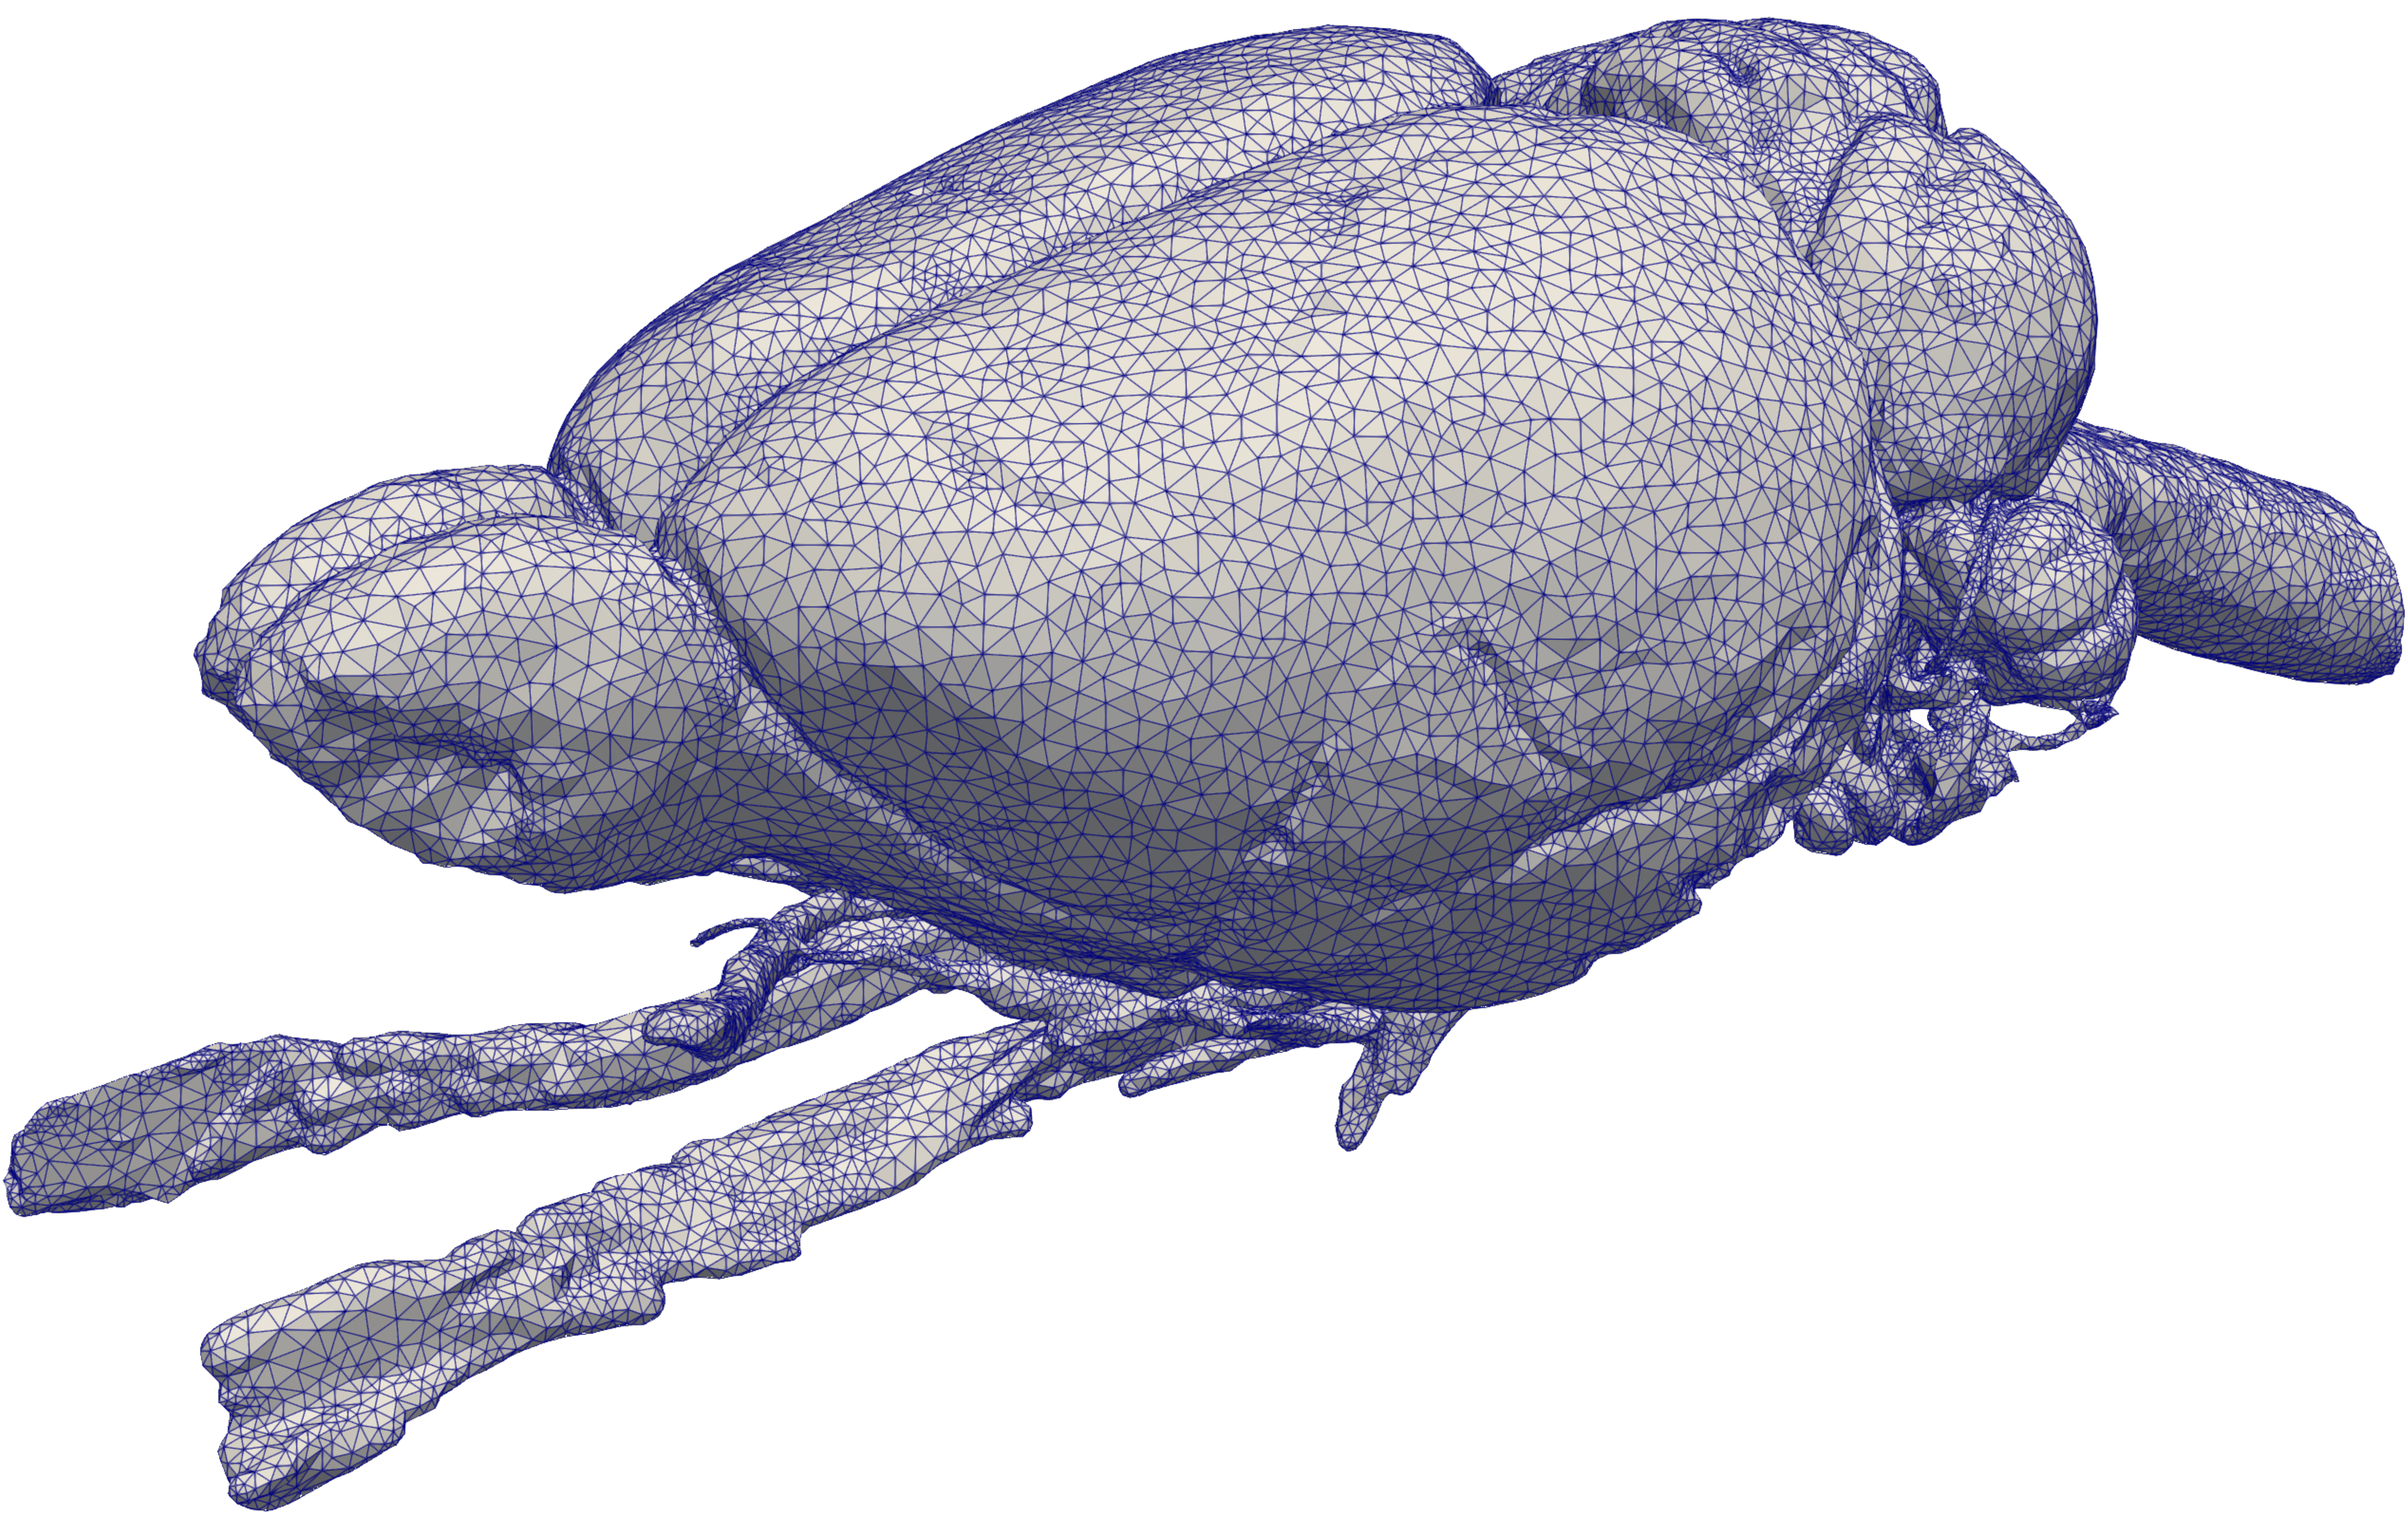
\includegraphics[width=\textwidth]{images/poster/ratbrain-mesh64-cropped.pdf}
        \caption{Mesh Illustration.}
    \end{subfigure}
    \hfill
    \begin{subfigure}[t]{0.45\textwidth}
        \centering
        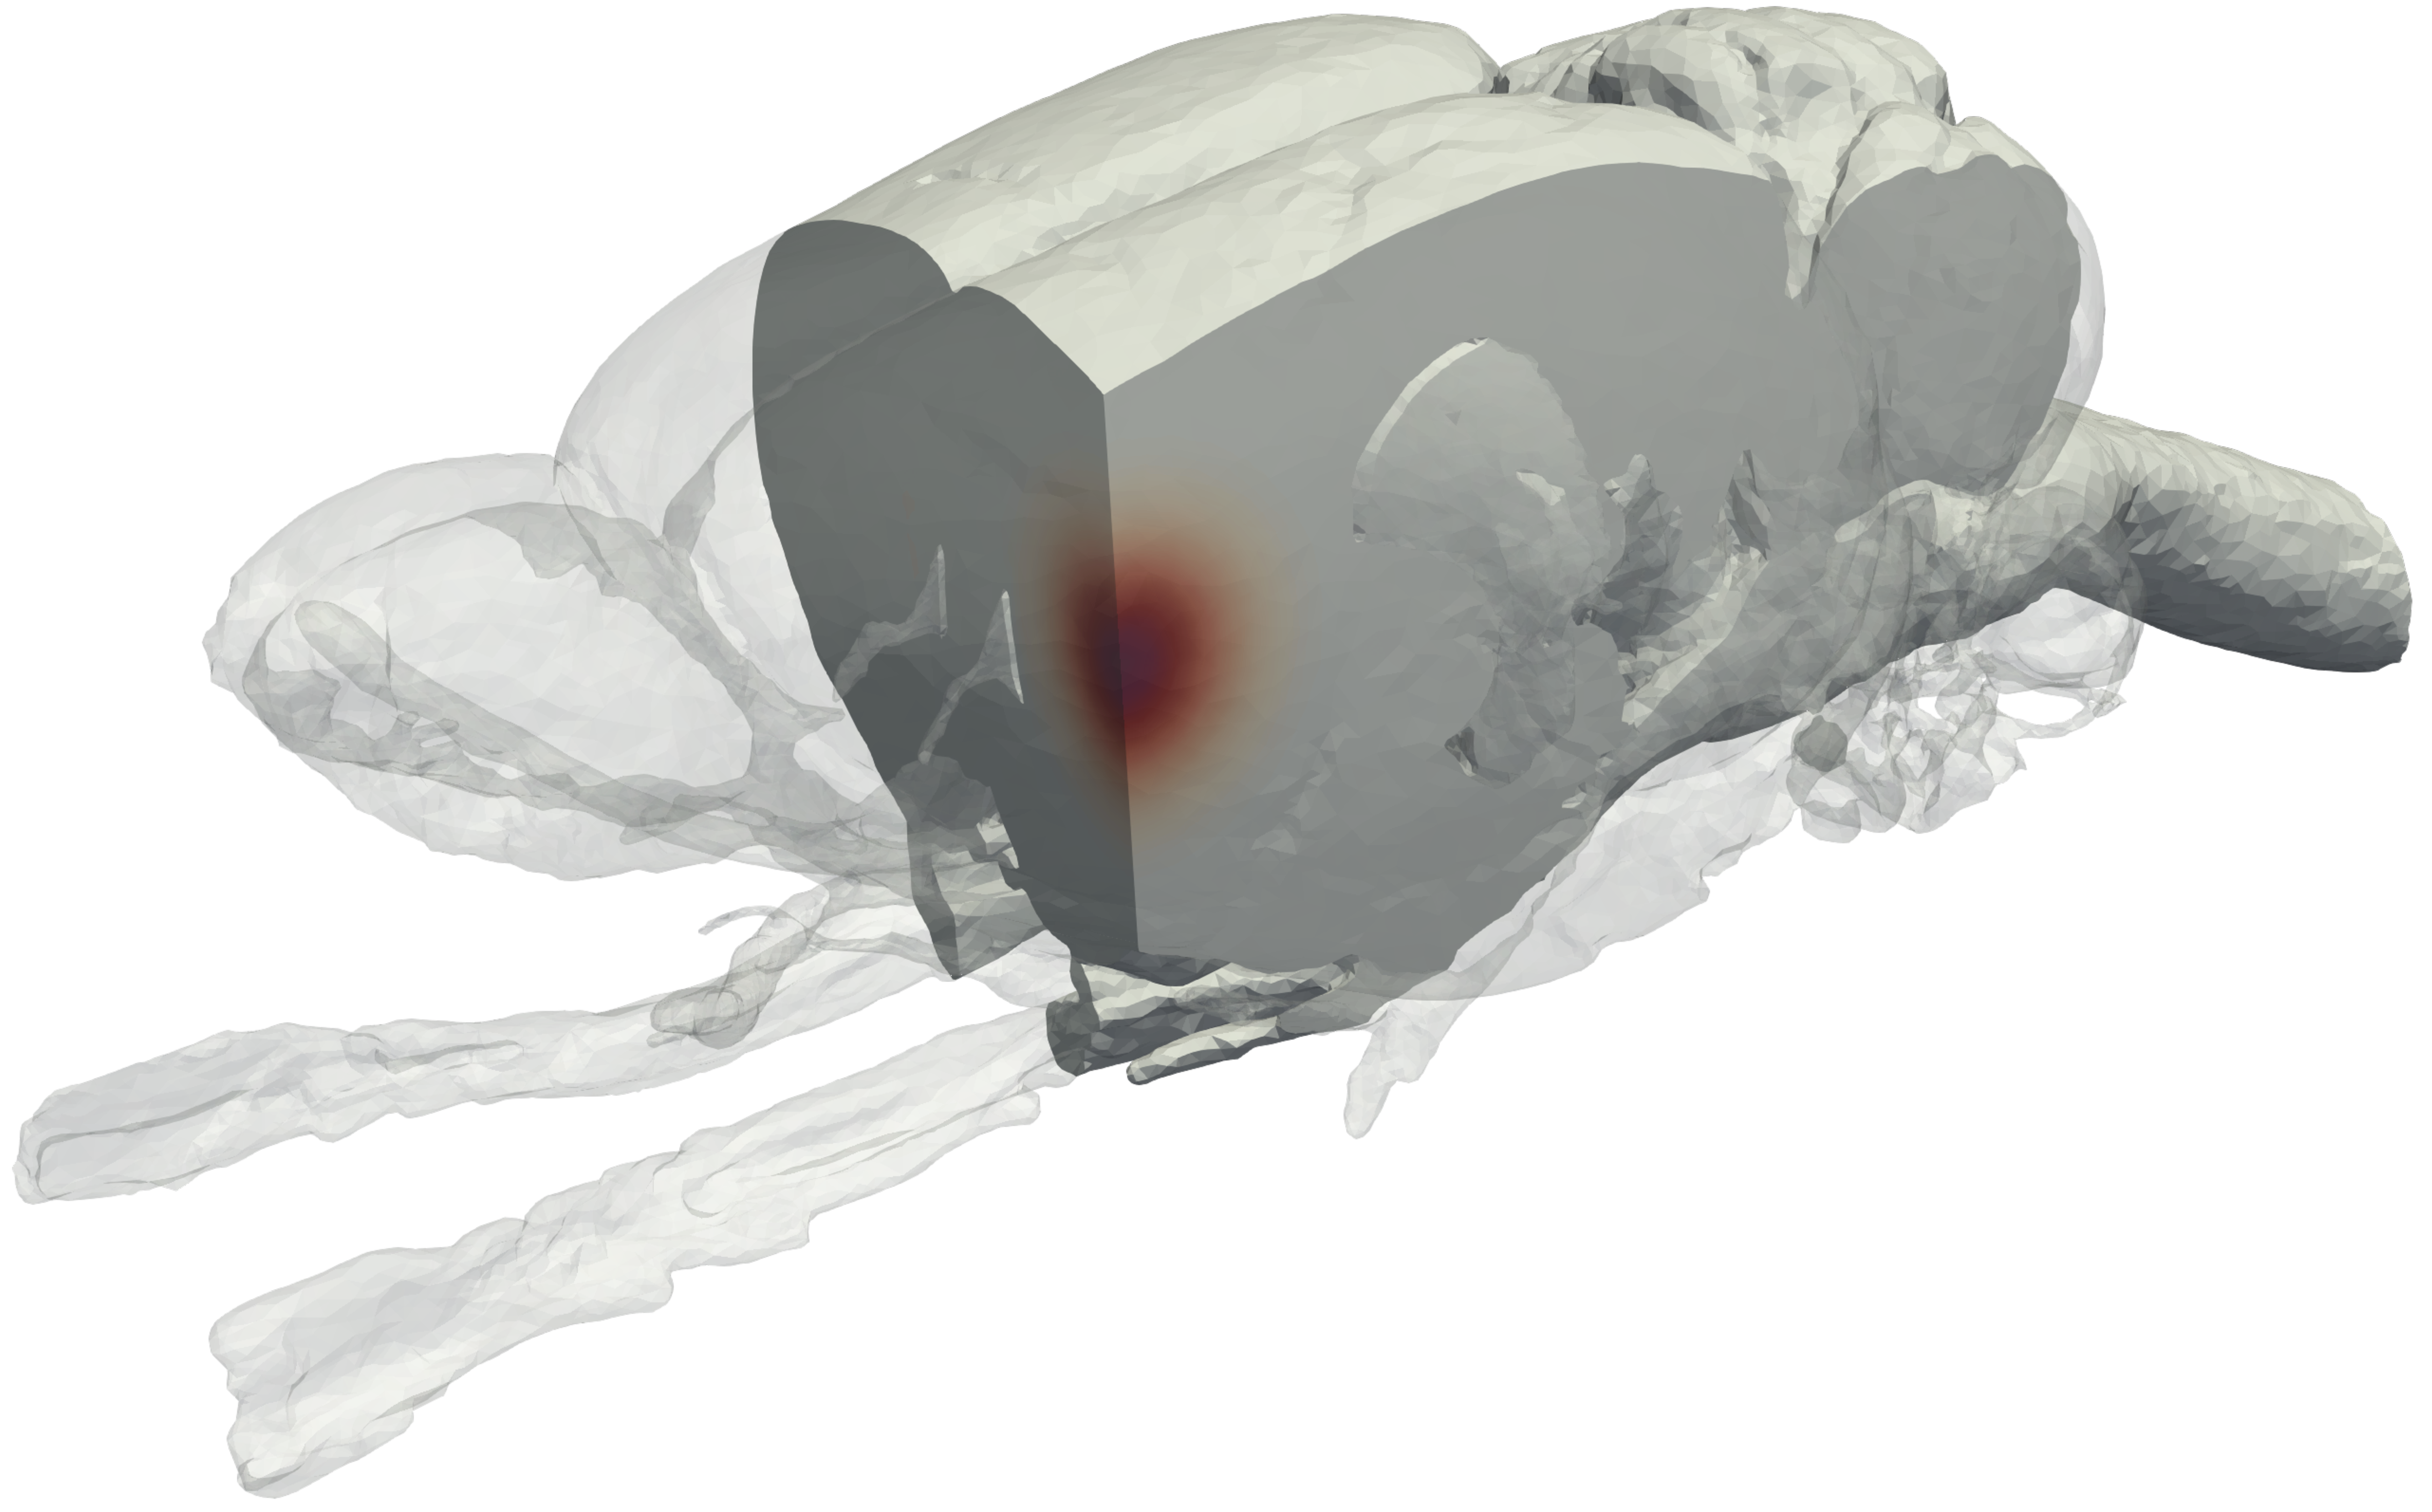
\includegraphics[width=\textwidth]{images/poster/ratbrain-initial-concentration-cropped.pdf}
        \caption{Initial Concentration}
    \end{subfigure}
    \hfill
    \caption{Illustration of the computational mesh and the initial condition for the concentration of \Cinulin.}
    \label{fig:mesh-illustration}
\end{figure}

For \textbf{\Cinulin test case 1}, we integrate the concentration in the extracellular space for different volumes. Indeed, to study how measurement variations made in the biological experiments could affect the results, we choose two possible integration domain: a cube embedded in the brain mesh to represent a measurement made in a sample of the brain and the total brain (see the results section~\ref{sec:results} to see these two domains). 

The relative mass of molecules in the extracellular space for the total brain at time $t$ is denoted by 
\[
c_{tot}(t) := \frac{\int_\Omega \phi_e c_e(t,\x) \, \dd \x }{ \int_\Omega \phi_e c_e(0,\x) \, \dd \x}.
\]
The relative mass of molecule within a cube $\omega$ centered around the injection point is indicated by 
\[
c_{\omega}(t) :=  \frac{\int_{\omega}  \phi_e c_e(t,\x) \, \dd \x }{\int_\omega  \phi_e c_e(0,\x) \, \dd \x}.  
\]

For the other test cases, we are interested in the same quantity but we also consider the molecules in the other compartments, leading to 
\[
c_{tot}(t) := \frac{\int_\Omega \sum_{j\in J}  \phi_j c_j(t,\x) \, \dd \x }{ \int_\Omega \phi_e c_e(0,\x) \, \dd \x}, \quad c_{\omega}(t) := \frac{\int_{\omega} \sum_{j\in J} \phi_j c_j(t,\x) \, \dd \x }{ \int_\omega \phi_e c_e(0,\x) \, \dd \x}.  
\]

We are also interested in measuring the velocity of the CSF in the different structures close to the pial surface.
From the solution of the pressure equations, we compute 
\begin{equation}
    \mathbf u_j = -\frac{\kappa_j}{\phi_j \mu_j}\nabla p_j, \quad j\in J, 
    \label{eq:velo}
\end{equation}
to obtain the velocity inside the $j$-th compartment. 

To compute the amount of fluid and transfer transmitted from one compartment to the another. To compute the mass of fluid transferring between compartment $j$ and compartment $i$, we use
\begin{equation}
Q_{ji} = \int_{\Omega} \rho \gamma_{j , i} \left( p_i - p_j \right)\, \dd \x,  
\label{eq:compute-transfer}
\end{equation}
with $\rho$ the constant mass density of the fluid in \si{g.mm^{-3}}. 
To compute the amount of exchange of CSF between the compartment $j$ and the SAS, we use 
\begin{equation}
Q_{j,\text{SAS}} = \int_{\partial \Omega} \rho_\text{CSF} \left(- \frac{\kappa_j}{ \mu_j}\nabla p_j  \cdot\pmb{\nu}\right) \,\dd s.\label{eq:compute-transfer-SAS}
\end{equation}


To compute the mass of molecules moving from from compartment $i$ to $j$, we have 
\begin{equation}
    M_{ji}(t) = \int_\Omega  \lambda_{j, i}( c_i- c_j) +  \frac{(c_j+c_i)}{2} \tilde \gamma_{j , i} (p_i - p_j-\sigma_{ij}(\pi_i-\pi_j))  \, \dd \x.
    \label{eq:matrixM}
\end{equation}
\subsection{Solution method and verification}

The spatial mesh used to produce the numerical results is presented in Appendix~\ref{app:mesh}. 
To solve the models~\eqref{eq:diffusion-convection} and~\eqref{eq:main-system} we use the finite element method for the discretization in space and an implicit Euler method to integrate in time the resulting ordinary differential systems. The details of the numerical scheme can be found in Appendix~\ref{app:model-num}. 
Details about what solving algorithm is used can be found in Appendix~\ref{app:mesh}.

In this section, we choose a resolution for the spatial mesh of $h=1/32$. The temporal domain is $[0,T]$ with $T=360 \si{min}$ with a time step $\dt = 1 \si{min}$. 
The numerical scheme has been implemented using the Fenics Library\cite{alnaes2015fenics,LoggMardalEtAl2012}. 







% Results and Discussion can be combined.
\section*{Results}
Nulla mi mi, venenatis sed ipsum varius, Table~\ref{table1} volutpat euismod diam. Proin rutrum vel massa non gravida. Quisque tempor sem et dignissim rutrum. Lorem ipsum dolor sit amet, consectetur adipiscing elit. Morbi at justo vitae nulla elementum commodo eu id massa. In vitae diam ac augue semper tincidunt eu ut eros. Fusce fringilla erat porttitor lectus cursus, vel sagittis arcu lobortis. Aliquam in enim semper, aliquam massa id, cursus neque. Praesent faucibus semper libero.

% Place tables after the first paragraph in which they are cited.
\begin{table}[!ht]
\begin{adjustwidth}{-2.25in}{0in} % Comment out/remove adjustwidth environment if table fits in text column.
\centering
\caption{
{\bf Table caption Nulla mi mi, venenatis sed ipsum varius, volutpat euismod diam.}}
\begin{tabular}{|l+l|l|l|l|l|l|l|}
\hline
\multicolumn{4}{|l|}{\bf Heading1} & \multicolumn{4}{|l|}{\bf Heading2}\\ \thickhline
$cell1 row1$ & cell2 row 1 & cell3 row 1 & cell4 row 1 & cell5 row 1 & cell6 row 1 & cell7 row 1 & cell8 row 1\\ \hline
$cell1 row2$ & cell2 row 2 & cell3 row 2 & cell4 row 2 & cell5 row 2 & cell6 row 2 & cell7 row 2 & cell8 row 2\\ \hline
$cell1 row3$ & cell2 row 3 & cell3 row 3 & cell4 row 3 & cell5 row 3 & cell6 row 3 & cell7 row 3 & cell8 row 3\\ \hline
\end{tabular}
\begin{flushleft} Table notes Phasellus venenatis, tortor nec vestibulum mattis, massa tortor interdum felis, nec pellentesque metus tortor nec nisl. Ut ornare mauris tellus, vel dapibus arcu suscipit sed.
\end{flushleft}
\label{table1}
\end{adjustwidth}
\end{table}


%PLOS does not support heading levels beyond the 3rd (no 4th level headings).
\subsection*{\lorem\ and \ipsum\ nunc blandit a tortor}
\subsubsection*{3rd level heading} 
Maecenas convallis mauris sit amet sem ultrices gravida. Etiam eget sapien nibh. Sed ac ipsum eget enim egestas ullamcorper nec euismod ligula. Curabitur fringilla pulvinar lectus consectetur pellentesque. Quisque augue sem, tincidunt sit amet feugiat eget, ullamcorper sed velit. Sed non aliquet felis. Lorem ipsum dolor sit amet, consectetur adipiscing elit. Mauris commodo justo ac dui pretium imperdiet. Sed suscipit iaculis mi at feugiat. 

\begin{enumerate}
	\item{react}
	\item{diffuse free particles}
	\item{increment time by dt and go to 1}
\end{enumerate}


\subsection*{Sed ac quam id nisi malesuada congue}

Nulla mi mi, venenatis sed ipsum varius, volutpat euismod diam. Proin rutrum vel massa non gravida. Quisque tempor sem et dignissim rutrum. Lorem ipsum dolor sit amet, consectetur adipiscing elit. Morbi at justo vitae nulla elementum commodo eu id massa. In vitae diam ac augue semper tincidunt eu ut eros. Fusce fringilla erat porttitor lectus cursus, vel sagittis arcu lobortis. Aliquam in enim semper, aliquam massa id, cursus neque. Praesent faucibus semper libero.

\begin{itemize}
	\item First bulleted item.
	\item Second bulleted item.
	\item Third bulleted item.
\end{itemize}

\section*{Discussion}
Nulla mi mi, venenatis sed ipsum varius, Table~\ref{table1} volutpat euismod diam. Proin rutrum vel massa non gravida. Quisque tempor sem et dignissim rutrum. Lorem ipsum dolor sit amet, consectetur adipiscing elit. Morbi at justo vitae nulla elementum commodo eu id massa. In vitae diam ac augue semper tincidunt eu ut eros. Fusce fringilla erat porttitor lectus cursus, vel sagittis arcu lobortis. Aliquam in enim semper, aliquam massa id, cursus neque. Praesent faucibus semper libero~\cite{bib3}.

\section*{Conclusion}

CO\textsubscript{2} Maecenas convallis mauris sit amet sem ultrices gravida. Etiam eget sapien nibh. Sed ac ipsum eget enim egestas ullamcorper nec euismod ligula. Curabitur fringilla pulvinar lectus consectetur pellentesque. Quisque augue sem, tincidunt sit amet feugiat eget, ullamcorper sed velit. 

Sed non aliquet felis. Lorem ipsum dolor sit amet, consectetur adipiscing elit. Mauris commodo justo ac dui pretium imperdiet. Sed suscipit iaculis mi at feugiat. Ut neque ipsum, luctus id lacus ut, laoreet scelerisque urna. Phasellus venenatis, tortor nec vestibulum mattis, massa tortor interdum felis, nec pellentesque metus tortor nec nisl. Ut ornare mauris tellus, vel dapibus arcu suscipit sed. Nam condimentum sem eget mollis euismod. Nullam dui urna, gravida venenatis dui et, tincidunt sodales ex. Nunc est dui, sodales sed mauris nec, auctor sagittis leo. Aliquam tincidunt, ex in facilisis elementum, libero lectus luctus est, non vulputate nisl augue at dolor. For more information, see \nameref{S1_Appendix}.

\section*{Supporting information}

% Include only the SI item label in the paragraph heading. Use the \nameref{label} command to cite SI items in the text.
\paragraph*{S1 Fig.}
\label{S1_Fig}
{\bf Bold the title sentence.} Add descriptive text after the title of the item (optional).

\paragraph*{S2 Fig.}
\label{S2_Fig}
{\bf Lorem ipsum.} Maecenas convallis mauris sit amet sem ultrices gravida. Etiam eget sapien nibh. Sed ac ipsum eget enim egestas ullamcorper nec euismod ligula. Curabitur fringilla pulvinar lectus consectetur pellentesque.

\paragraph*{S1 File.}
\label{S1_File}
{\bf Lorem ipsum.}  Maecenas convallis mauris sit amet sem ultrices gravida. Etiam eget sapien nibh. Sed ac ipsum eget enim egestas ullamcorper nec euismod ligula. Curabitur fringilla pulvinar lectus consectetur pellentesque.

\paragraph*{S1 Video.}
\label{S1_Video}
{\bf Lorem ipsum.}  Maecenas convallis mauris sit amet sem ultrices gravida. Etiam eget sapien nibh. Sed ac ipsum eget enim egestas ullamcorper nec euismod ligula. Curabitur fringilla pulvinar lectus consectetur pellentesque.

\paragraph*{S1 Appendix.}
\label{S1_Appendix}
{\bf Lorem ipsum.} Maecenas convallis mauris sit amet sem ultrices gravida. Etiam eget sapien nibh. Sed ac ipsum eget enim egestas ullamcorper nec euismod ligula. Curabitur fringilla pulvinar lectus consectetur pellentesque.

\paragraph*{S1 Table.}
\label{S1_Table}
{\bf Lorem ipsum.} Maecenas convallis mauris sit amet sem ultrices gravida. Etiam eget sapien nibh. Sed ac ipsum eget enim egestas ullamcorper nec euismod ligula. Curabitur fringilla pulvinar lectus consectetur pellentesque.

\section*{Acknowledgments}
Cras egestas velit mauris, eu mollis turpis pellentesque sit amet. Interdum et malesuada fames ac ante ipsum primis in faucibus. Nam id pretium nisi. Sed ac quam id nisi malesuada congue. Sed interdum aliquet augue, at pellentesque quam rhoncus vitae.

\nolinenumbers

% Either type in your references using
\begin{thebibliography}{10}

\bibitem{abbott2004evidence}
{\sc N.~J. Abbott}, {\em Evidence for bulk flow of brain interstitial fluid:
  significance for physiology and pathology}, Neurochemistry international, 45
  (2004), pp.~545--552.

\bibitem{abbott_role_2018}
{\sc N.~J. Abbott, M.~E. Pizzo, J.~E. Preston, D.~Janigro, and R.~G. Thorne},
  {\em The role of brain barriers in fluid movement in the {CNS}: is there a
  ‘glymphatic’ system?}, Acta Neuropathol, 135 (2018), pp.~387--407.

\bibitem{cgal:rty-m3-22a}
{\sc P.~Alliez, C.~Jamin, L.~Rineau, S.~Tayeb, J.~Tournois, and M.~Yvinec},
  {\em {3D} mesh generation}, in {CGAL} User and Reference Manual, {CGAL
  Editorial Board}, {5.4}~ed., 2022.

\bibitem{alnaes2015fenics}
{\sc M.~S. {Aln{\ae}s}, J.~Blechta, J.~E. {Hake}, A.~Johansson, B.~Kehlet,
  A.~Logg, C.~Richardson, J.~Ring, M.~E. {Rognes}, and G.~N. {Wells}}, {\em The
  fenics project version 1.5}, Archive of Numerical Software, 3 (2015).

\bibitem{asgari_glymphatic_2016}
{\sc M.~Asgari, D.~de~Zélicourt, and V.~Kurtcuoglu}, {\em Glymphatic solute
  transport does not require bulk flow}, Sci Rep, 6 (2016), p.~38635.
\newblock Number: 1 Publisher: Nature Publishing Group.

\bibitem{Bai-MPET-1993}
{\sc M.~Bai, D.~Elsworth, and J.-C. Roegiers}, {\em
  Multiporosity/multipermeability approach to the simulation of naturally
  fractured reservoirs}, Water Resources Research, 29 (1993), pp.~1621--1633.

\bibitem{Bai_1993_Multiporosity}
\leavevmode\vrule height 2pt depth -1.6pt width 23pt, {\em
  Multiporosity/multipermeability approach to the simulation of naturally
  fractured reservoirs}, Water Resources Research, 29 (1993), pp.~1621--1633.

\bibitem{baker_membrane_2012}
{\sc R.~W. Baker}, {\em Membrane technology and applications}, John Wiley \&
  Sons, Chichester, West Sussex ; Hoboken, 3rd ed~ed., 2012.

\bibitem{bakker2019paravascular}
{\sc E.~N. Bakker, D.~M. Naessens, and E.~VanBavel}, {\em Paravascular spaces:
  entry to or exit from the brain?}, Experimental physiology, 104 (2019),
  pp.~1013--1017.

\bibitem{BALLERINI2020102120}
{\sc L.~Ballerini, T.~Booth, M.~del C.~{Valdés Hernández}, S.~Wiseman,
  R.~Lovreglio, S.~{Muñoz Maniega}, Z.~Morris, A.~Pattie, J.~Corley, A.~Gow,
  M.~E. Bastin, I.~J. Deary, and J.~Wardlaw}, {\em Computational quantification
  of brain perivascular space morphologies: Associations with vascular risk
  factors and white matter hyperintensities. a study in the lothian birth
  cohort 1936}, NeuroImage: Clinical, 25 (2020), p.~102120.

\bibitem{bedussi-2018-paravascular}
{\sc B.~Bedussi, M.~Almasian, J.~de~Vos, E.~VanBavel, and E.~N. Bakker}, {\em
  Paravascular spaces at the brain surface: Low resistance pathways for
  cerebrospinal fluid flow}, Journal of Cerebral Blood Flow \& Metabolism, 38
  (2018), pp.~719--726.
\newblock PMID: 29039724.

\bibitem{Biot-1941-Consolidation}
{\sc M.~A. Biot}, {\em General theory of three‐dimensional consolidation},
  Journal of Applied Physics, 12 (1941), pp.~155--164.

\bibitem{Biot-1955-Consolidation2}
{\sc M.~A. Biot}, {\em Theory of elasticity and consolidation for a porous
  anisotropic solid}, Journal of Applied Physics, 26 (1955), pp.~182--185.

\bibitem{bloomfield1998effects}
{\sc I.~Bloomfield, I.~Johnston, and L.~Bilston}, {\em Effects of proteins,
  blood cells and glucose on the viscosity of cerebrospinal fluid}, Pediatric
  neurosurgery, 28 (1998), pp.~246--251.

\bibitem{croci2019uncertainty}
{\sc M.~Croci, V.~Vinje, and M.~E. Rognes}, {\em Uncertainty quantification of
  parenchymal tracer distribution using random diffusion and convective
  velocity fields}, Fluids and Barriers of the CNS, 16 (2019), pp.~1--21.

\bibitem{Cserr-1991-Extracellular}
{\sc H.~F. Cserr, M.~DePasquale, C.~Nicholson, C.~S. Patlak, K.~D. Pettigrew,
  and M.~E. Rice}, {\em Extracellular volume decreases while cell volume is
  maintained by ion uptake in rat brain during acute hypernatremia.}, The
  Journal of Physiology, 442 (1991), pp.~277--295.

\bibitem{dreyer2022}
{\sc L.~W. Dreyer}, {\em Normal pressure with abnormal geometry - a
  biomechanical model of normal pressure hydrocephalus during infusion tests},
  Ms. Thesis, Department of Mathematics, University of Oslo,  (2022).

\bibitem{el-bouri-conferencepaper}
{\sc W.~El-Bouri, Y.~Bing, T.~Józsa, and S.~Payne}, {\em A novel multi-scale,
  multi-compartment model of oxygen transport - towards in-silico clinical
  trials in the entire human brain}, 09 2019.

\bibitem{el2019coupled}
{\sc W.~El-Bouri, Y.~Bing, and S.~Payne}, {\em A coupled multi-compartment
  model of blood and oxygen transport in the human cerebral cortex}, JOURNAL OF
  CEREBRAL BLOOD FLOW AND METABOLISM, 39 (2019), pp.~300--301.

\bibitem{Payne-clot-2021}
{\sc W.~K. El-Bouri, A.~MacGowan, T.~I. Józsa, M.~J. Gounis, and S.~J. Payne},
  {\em Modelling the impact of clot fragmentation on the microcirculation after
  thrombectomy}, PLOS Computational Biology, 17 (2021), pp.~1--25.

\bibitem{eliseussen2021posteriori}
{\sc E.~Eliseussen, M.~E. Rognes, and T.~B. Thompson}, {\em A-posteriori error
  estimation and adaptivity for multiple-network poroelasticity}, arXiv
  preprint arXiv:2111.13456,  (2021).

\bibitem{Erbertseder-2012-lung}
{\sc K.~Erbertseder, J.~Reichold, B.~Flemisch, P.~Jenny, and R.~Helmig}, {\em A
  coupled discrete/continuum model for describing cancer-therapeutic transport
  in the lung}, PLOS ONE, 7 (2012), pp.~1--17.

\bibitem{farkas-diam-capillaries}
{\sc E.~Farkas and P.~G. Luiten}, {\em Cerebral microvascular pathology in
  aging and alzheimer's disease}, Progress in Neurobiology, 64 (2001),
  pp.~575--611.

\bibitem{fedorov2012}
{\sc A.~Fedorov, R.~Beichel, J.~Kalpathy-cramer, J.~Finet, J.~christophe
  Fillion-robin, S.~Pujol, C.~Bauer, D.~Jennings, F.~Fennessy, M.~Sonka,
  J.~Buatti, S.~Aylward, J.~V. Miller, S.~Pieper, and R.~Kikinis}, {\em 3d
  slicer as an image computing platform for the quantitative imaging network},
  Magnetic Resonance Imaging, 30 (2012), pp.~1323--1341.

\bibitem{fraser1990measurement}
{\sc P.~Fraser, A.~D. Dallas, and S.~Davies}, {\em Measurement of filtration
  coefficient in single cerebral microvessels of the frog.}, The Journal of
  physiology, 423 (1990), pp.~343--361.

\bibitem{Guo-2019-MPET}
{\sc L.~Guo, Z.~Li, J.~Lyu, Y.~Mei, J.~C. Vardakis, D.~Chen, C.~Han, X.~Lou,
  and Y.~Ventikos}, {\em On the validation of a multiple-network poroelastic
  model using arterial spin labeling mri data}, Frontiers in Computational
  Neuroscience, 13 (2019).

\bibitem{Guo-2018-MPET}
{\sc L.~Guo, J.~C. Vardakis, T.~Lassila, M.~Mitolo, N.~Ravikumar, D.~Chou,
  M.~Lange, A.~Sarrami-Foroushani, B.~J. Tully, Z.~A. Taylor, S.~Varma,
  A.~Venneri, A.~F. Frangi, and Y.~Ventikos}, {\em Subject-specific
  multi-poroelastic model for exploring the risk factors associated with the
  early stages of alzheimer's disease}, Interface Focus, 8 (2018), p.~20170019.

\bibitem{Holter9894}
{\sc K.~E. Holter, B.~Kehlet, A.~Devor, T.~J. Sejnowski, A.~M. Dale, S.~W.
  Omholt, O.~P. Ottersen, E.~A. Nagelhus, K.-A. Mardal, and K.~H. Pettersen},
  {\em Interstitial solute transport in 3d reconstructed neuropil occurs by
  diffusion rather than bulk flow}, Proceedings of the National Academy of
  Sciences, 114 (2017), pp.~9894--9899.

\bibitem{hornkjol2022csf}
{\sc M.~Hornkjol, L.~M. Valnes, G.~Ringstad, M.~E. Rognes, P.~K. Eide, K.-A.
  Mardal, and V.~Vinje}, {\em Csf circulation and dispersion yield rapid
  clearance from intracranial compartments}, bioRxiv,  (2022).

\bibitem{Hornung-1996-homogenization}
{\sc U.~Hornung}, ed., {\em Homogenization and Porous Media}, Springer-Verlag,
  Berlin, Heidelberg, 1996.

\bibitem{Iliff_2012_PVS}
{\sc J.~J. Iliff, M.~Wang, Y.~Liao, B.~A. Plogg, W.~Peng, G.~A. Gundersen,
  H.~Benveniste, G.~E. Vates, R.~Deane, S.~A. Goldman, E.~A. Nagelhus, and
  M.~Nedergaard}, {\em A paravascular pathway facilitates csf flow through the
  brain parenchyma and the clearance of interstitial solutes, including amyloid
  \&\#x3b2;}, Science Translational Medicine, 4 (2012), pp.~147ra111--147ra111.

\bibitem{jessen_glymphatic_2015}
{\sc N.~A. Jessen, A.~S.~F. Munk, I.~Lundgaard, and M.~Nedergaard}, {\em The
  {Glymphatic} {System}: {A} {Beginner}’s {Guide}}, Neurochem Res, 40 (2015),
  pp.~2583--2599.

\bibitem{jozsa2021sensitivity}
{\sc T.~I. J{\'o}zsa, R.~M. Padmos, W.~K. El-Bouri, A.~G. Hoekstra, and S.~J.
  Payne}, {\em On the sensitivity analysis of porous finite element models for
  cerebral perfusion estimation}, Annals of Biomedical Engineering, 49 (2021),
  pp.~3647--3665.

\bibitem{jozsa2021porous}
{\sc T.~I. J{\'o}zsa, R.~M. Padmos, N.~Samuels, W.~El-Bouri, A.~G. Hoekstra,
  and S.~J. Payne}, {\em A porous circulation model of the human brain for in
  silico clinical trials in ischaemic stroke}, Interface Focus, 11 (2021),
  p.~20190127.

\bibitem{Levick-1991-Capillary}
{\sc L.~JR}, {\em Capillary filtration-absorption balance reconsidered in light
  of dynamic extravascular factors}, Experimental Physiology, 76 (1991),
  pp.~825--857.

\bibitem{kedem-1958-thermo}
{\sc O.~Kedem and A.~Katchalsky}, {\em Thermodynamic analysis of the
  permeability of biological membranes to non-electrolytes}, Biochimica et
  Biophysica Acta, 27 (1958), pp.~229--246.

\bibitem{kimura1993measurement}
{\sc M.~Kimura, H.~H. Dietrich, V.~H. Huxley, D.~R. Reichner, and R.~G. Dacey},
  {\em Measurement of hydraulic conductivity in isolated arterioles of rat
  brain cortex}, American Journal of Physiology-Heart and Circulatory
  Physiology, 264 (1993), pp.~H1788--H1797.
\newblock PMID: 8322907.

\bibitem{lai1983sampling}
{\sc Y.~Lai, P.~Smith, W.~Lamm, and J.~Hildebrandt}, {\em Sampling and analysis
  of cerebrospinal fluid for chronic studies in awake rats}, Journal of Applied
  Physiology, 54 (1983), pp.~1754--1757.

\bibitem{lanman1971diffusion}
{\sc R.~C. Lanman, J.~A. Burton, and L.~S. Schanker}, {\em Diffusion
  coefficients of some 14c-labeled saccharides of biological interest}, Life
  Sciences, 10 (1971), pp.~803--811.

\bibitem{Lee-2001-CBV}
{\sc S.-P. Lee, T.~Q. Duong, G.~Yang, C.~Iadecola, and S.-G. Kim}, {\em
  Relative changes of cerebral arterial and venous blood volumes during
  increased cerebral blood flow: Implications for bold fmri}, Magnetic
  Resonance in Medicine, 45 (2001), pp.~791--800.

\bibitem{li2010permeability}
{\sc G.~Li, M.~J. Simon, L.~M. Cancel, Z.-D. Shi, X.~Ji, J.~M. Tarbell,
  B.~Morrison, and B.~M. Fu}, {\em Permeability of endothelial and astrocyte
  cocultures: in vitro blood--brain barrier models for drug delivery studies},
  Annals of biomedical engineering, 38 (2010), pp.~2499--2511.

\bibitem{Li-2010-model}
{\sc G.~Li, W.~Yuan, and B.~M. Fu}, {\em A model for the blood–brain barrier
  permeability to water and small solutes}, Journal of Biomechanics, 43 (2010),
  pp.~2133--2140.

\bibitem{li-2010-BBB}
\leavevmode\vrule height 2pt depth -1.6pt width 23pt, {\em A model for the
  blood–brain barrier permeability to water and small solutes}, Journal of
  Biomechanics, 43 (2010), pp.~2133--2140.

\bibitem{LoggMardalEtAl2012}
{\sc A.~Logg, K.-A. Mardal, G.~N. Wells, et~al.}, {\em Automated Solution of
  Differential Equations by the Finite Element Method}, Springer, 2012.

\bibitem{Mardal-2022-mri}
{\sc K.-A. Mardal, M.~Rognes, T.~Thompson, and L.~Valnes}, {\em Mathematical
  Modeling of the Human Brain: From Magnetic Resonance Images to Finite Element
  Simulation}, Springer, Cham, 01 2022.

\bibitem{mayhan_role_1986}
{\sc W.~G. Mayhan and D.~D. Heistad}, {\em Role of veins and cerebral venous
  pressure in disruption of the blood-brain barrier}, Circ Res, 59 (1986),
  pp.~216--220.

\bibitem{mestre_flow_2018}
{\sc H.~Mestre, J.~Tithof, T.~Du, W.~Song, W.~Peng, A.~M. Sweeney, G.~Olveda,
  J.~H. Thomas, M.~Nedergaard, and D.~H. Kelley}, {\em Flow of cerebrospinal
  fluid is driven by arterial pulsations and is reduced in hypertension}, Nat
  Commun, 9 (2018), p.~4878.
\newblock Number: 1 Publisher: Nature Publishing Group.

\bibitem{Michel-1999-permeablity}
{\sc C.~C. Michel and F.~E. Curry}, {\em Microvascular permeability},
  Physiological Reviews, 79 (1999), pp.~703--761.
\newblock PMID: 10390517.

\bibitem{Muir-2008-CBF}
{\sc E.~R. Muir, Q.~Shen, and T.~Q. Duong}, {\em Cerebral blood flow mri in
  mice using the cardiac-spin-labeling technique}, Magnetic Resonance in
  Medicine, 60 (2008), pp.~744--748.

\bibitem{murtha2014cerebrospinal}
{\sc L.~A. Murtha, Q.~Yang, M.~W. Parsons, C.~R. Levi, D.~J. Beard, N.~J.
  Spratt, and D.~D. McLeod}, {\em Cerebrospinal fluid is drained primarily via
  the spinal canal and olfactory route in young and aged spontaneously
  hypertensive rats}, Fluids and Barriers of the CNS, 11 (2014), pp.~1--9.

\bibitem{nag2011nature}
{\sc S.~Nag, B.~Sarkar, A.~Bandyopadhyay, B.~Sahoo, V.~K. Sreenivasan,
  M.~Kombrabail, C.~Muralidharan, and S.~Maiti}, {\em Nature of the
  amyloid-$\beta$ monomer and the monomer-oligomer equilibrium}, Journal of
  Biological Chemistry, 286 (2011), pp.~13827--13833.

\bibitem{nagy_basic_2018}
{\sc E.~Nagy}, {\em Basic {Equations} of {Mass} {Transport} {Through} a
  {Membrane} {Layer}}, Elsevier, Nov. 2018.

\bibitem{Al-arterial-diam}
{\sc A.~C. Ngai and H.~R. Winn}, {\em Modulation of cerebral arteriolar
  diameter by intraluminal flow and pressure}, Circulation Research, 77 (1995),
  pp.~832--840.

\bibitem{Nguyen-venule-diam}
{\sc J.~Nguyen, N.~Nishimura, R.~N. Fetcho, C.~Iadecola, and C.~B. Schaffer},
  {\em Occlusion of cortical ascending venules causes blood flow decreases,
  reversals in flow direction, and vessel dilation in upstream capillaries},
  Journal of Cerebral Blood Flow \& Metabolism, 31 (2011), pp.~2243--2254.
\newblock PMID: 21712834.

\bibitem{nicholson2001diffusion}
{\sc C.~Nicholson}, {\em Diffusion and related transport mechanisms in brain
  tissue}, Reports on progress in Physics, 64 (2001), p.~815.

\bibitem{nicholson-1981-ion}
{\sc C.~Nicholson and J.~M. Phillips}, {\em Ion diffusion modified by
  tortuosity and volume fraction in the extracellular microenvironment of the
  rat cerebellum.}, The Journal of Physiology, 321 (1981), pp.~225--257.

\bibitem{papp2014}
{\sc E.~A. Papp, T.~B. Leergaard, E.~Calabrese, G.~A. Johnson, and J.~G.
  Bjaalie}, {\em Waxholm space atlas of the sprague dawley rat brain},
  {NeuroImage}, 97 (2014), pp.~374--386.

\bibitem{pardridge2011drug}
{\sc W.~M. Pardridge}, {\em Drug transport in brain via the cerebrospinal
  fluid}, Fluids and Barriers of the CNS, 8 (2011), pp.~1--4.

\bibitem{Penta-homogenization-2015}
{\sc R.~Penta, D.~Ambrosi, and A.~Quarteroni}, {\em Multiscale homogenization
  for fluid and drug transport in vascularized malignant tissues}, Mathematical
  Models and Methods in Applied Sciences, 25 (2015), pp.~79--108.

\bibitem{Adriana-2007-MR}
{\sc A.~T. Perles-Barbacaru and H.~Lahrech}, {\em A new magnetic resonance
  imaging method for mapping the cerebral blood volume fraction: The rapid
  steady-state t1 method}, Journal of Cerebral Blood Flow \& Metabolism, 27
  (2007), pp.~618--631.
\newblock PMID: 16850031.

\bibitem{proulx2021cerebrospinal}
{\sc S.~T. Proulx}, {\em Cerebrospinal fluid outflow: a review of the
  historical and contemporary evidence for arachnoid villi, perineural routes,
  and dural lymphatics}, Cellular and Molecular Life Sciences, 78 (2021),
  pp.~2429--2457.

\bibitem{ray_analysis_2019}
{\sc L.~Ray, J.~J. Iliff, and J.~J. Heys}, {\em Analysis of convective and
  diffusive transport in the brain interstitium}, Fluids Barriers CNS, 16
  (2019), pp.~1--18.
\newblock Number: 1 Publisher: BioMed Central.

\bibitem{ray2021quantitative}
{\sc L.~A. Ray, M.~Pike, M.~Simon, J.~J. Iliff, and J.~J. Heys}, {\em
  Quantitative analysis of macroscopic solute transport in the murine brain},
  Fluids and Barriers of the CNS, 18 (2021), pp.~1--19.

\bibitem{reeves_glymphatic_2020}
{\sc B.~C. Reeves, J.~K. Karimy, A.~J. Kundishora, H.~Mestre, H.~M. Cerci,
  C.~Matouk, S.~L. Alper, I.~Lundgaard, M.~Nedergaard, and K.~T. Kahle}, {\em
  Glymphatic {System} {Impairment} in {Alzheimer}’s {Disease} and
  {Idiopathic} {Normal} {Pressure} {Hydrocephalus}}, Trends in Molecular
  Medicine, 26 (2020), pp.~285--295.
\newblock Publisher: Elsevier.

\bibitem{roberts2009ppar}
{\sc T.~J. Roberts, A.~C. Chapman, and M.~J. Cipolla}, {\em Ppar-$\gamma$
  agonist rosiglitazone reverses increased cerebral venous hydraulic
  conductivity during hypertension}, American Journal of Physiology-Heart and
  Circulatory Physiology, 297 (2009), pp.~H1347--H1353.

\bibitem{Roy-rat-pressure-2013}
{\sc U.~Roy~Chowdhury, B.~H. Holman, and M.~P. Fautsch}, {\em A novel rat model
  to study the role of intracranial pressure modulation on optic neuropathies},
  PLOS ONE, 8 (2013), p.~null.

\bibitem{Schultz-hydro-radii-1961}
{\sc S.~G. Schultz and A.~K. Solomon}, {\em {Determination of the Effective
  Hydrodynamic Radii of Small Molecules by Viscometry }}, Journal of General
  Physiology, 44 (1961), pp.~1189--1199.

\bibitem{shi-2014-Quantification}
{\sc L.~Shi, M.~Zeng, Y.~Sun, and B.~M. Fu}, {\em {Quantification of
  Blood-Brain Barrier Solute Permeability and Brain Transport by Multiphoton
  Microscopy}}, Journal of Biomechanical Engineering, 136 (2014).
\newblock 031005.

\bibitem{shibata2000clearance}
{\sc M.~Shibata, S.~Yamada, S.~R. Kumar, M.~Calero, J.~Bading, B.~Frangione,
  D.~M. Holtzman, C.~A. Miller, D.~K. Strickland, J.~Ghiso, et~al.}, {\em
  Clearance of alzheimer’s amyloid-$\beta$ 1-40 peptide from brain by ldl
  receptor--related protein-1 at the blood-brain barrier}, The Journal of
  clinical investigation, 106 (2000), pp.~1489--1499.

\bibitem{shipley_multiscale_2010}
{\sc R.~J. Shipley and S.~J. Chapman}, {\em Multiscale {Modelling} of {Fluid}
  and {Drug} {Transport} in {Vascular} {Tumours}}, Bull. Math. Biol., 72
  (2010), pp.~1464--1491.

\bibitem{shipley-four-comp}
{\sc R.~J. Shipley, P.~W. Sweeney, S.~J. Chapman, and T.~Roose}, {\em A
  four-compartment multiscale model of fluid and drug distribution in vascular
  tumours}, International Journal for Numerical Methods in Biomedical
  Engineering, 36 (2020), p.~e3315.

\bibitem{smith2019going}
{\sc A.~J. Smith and A.~S. Verkman}, {\em Going against the flow: Interstitial
  solute transport in brain is diffusive and aquaporin-4 independent}, The
  Journal of physiology, 597 (2019), p.~4421.

\bibitem{smith2007interstitial}
{\sc J.~H. Smith and J.~A. Humphrey}, {\em Interstitial transport and
  transvascular fluid exchange during infusion into brain and tumor tissue},
  Microvascular research, 73 (2007), pp.~58--73.

\bibitem{Strazielle-2000-invitro}
{\sc N.~Strazielle, J.-F. Ghersi-Egea, J.~Ghiso, M.-P. Dehouck, B.~Frangione,
  C.~Patlak, J.~Fenstermacher, and P.~Gorevic}, {\em {In Vitro Evidence That
  $\beta$-Amyloid Peptide $1–40$ Diffuses Across the Blood–Brain Barrier
  and Affects Its Permeability}}, Journal of Neuropathology \& Experimental
  Neurology, 59 (2000), pp.~29--38.

\bibitem{stoverud_modeling_2012}
{\sc K.~H. Støverud, M.~Darcis, R.~Helmig, and S.~M. Hassanizadeh}, {\em
  Modeling {Concentration} {Distribution} and {Deformation} {During}
  {Convection}-{Enhanced} {Drug} {Delivery} into {Brain} {Tissue}}, Transp
  Porous Med, 92 (2012), pp.~119--143.

\bibitem{thomas2022theoretical}
{\sc J.~H. Thomas}, {\em Theoretical analysis of wake/sleep changes in brain
  solute transport suggests a flow of interstitial fluid}, Fluids and Barriers
  of the CNS, 19 (2022), pp.~1--5.

\bibitem{tithof-2022-glymphatic}
{\sc J.~Tithof, K.~A. Boster, P.~A. Bork, M.~Nedergaard, J.~H. Thomas, and
  D.~H. Kelley}, {\em A network model of glymphatic flow under different
  experimentally-motivated parametric scenarios}, iScience, 25 (2022),
  p.~104258.

\bibitem{trainor1982transcapillary}
{\sc C.~Trainor and M.~Silverman}, {\em Transcapillary exchange of molecular
  weight markers in the postglomerular circulation: application of a
  barrier-limited model}, American Journal of Physiology-Renal Physiology, 242
  (1982), pp.~F436--F446.

\bibitem{tully_ventikos_2011}
{\sc B.~TULLY and Y.~VENTIKOS}, {\em Cerebral water transport using
  multiple-network poroelastic theory: application to normal pressure
  hydrocephalus}, Journal of Fluid Mechanics, 667 (2011), p.~188–215.

\bibitem{valnes_apparent_2020}
{\sc L.~M. Valnes, S.~K. Mitusch, G.~Ringstad, P.~K. Eide, S.~W. Funke, and
  K.-A. Mardal}, {\em Apparent diffusion coefficient estimates based on 24
  hours tracer movement support glymphatic transport in human cerebral cortex},
  Sci Rep, 10 (2020), p.~9176.

\bibitem{Vardakis-2016-cerebral}
{\sc J.~C. Vardakis, D.~Chou, B.~J. Tully, C.~C. Hung, T.~H. Lee, P.-H. Tsui,
  and Y.~Ventikos}, {\em Investigating cerebral oedema using poroelasticity},
  Medical Engineering \& Physics, 38 (2016), pp.~48--57.
\newblock Micro and Nano Flows 2014 (MNF2014) - Biomedical Stream.

\bibitem{Vinje-2020-ICP}
{\sc V.~Vinje, A.~Eklund, K.-A. Mardal, M.~E. {Rognes}, and K.-H. St{\o}verud},
  {\em Intracranial pressure elevation alters csf clearance pathways}, Fluids
  and Barriers of the CNS, 17 (2020).

\bibitem{Waters-2011-AB}
{\sc J.~Waters}, {\em The concentration of soluble extracellular
  amyloid-$\beta$ protein in acute brain slices from crnd8 mice}, PLOS ONE, 5
  (2011), pp.~1--16.

\bibitem{Wiig-1983-interstitial}
{\sc H.~Wiig and R.~K. Reed}, {\em Rat brain interstitial fluid pressure
  measured with micropipettes}, American Journal of Physiology-Heart and
  Circulatory Physiology, 244 (1983), pp.~H239--H246.
\newblock PMID: 6401940.

\bibitem{Xie_2013_sleep}
{\sc L.~Xie, H.~Kang, Q.~Xu, M.~J. Chen, Y.~Liao, M.~Thiyagarajan,
  J.~O’Donnell, D.~J. Christensen, C.~Nicholson, J.~J. Iliff, T.~Takano,
  R.~Deane, and M.~Nedergaard}, {\em Sleep drives metabolite clearance from the
  adult brain}, Science, 342 (2013), pp.~373--377.

\end{thebibliography}
%
% or
%
% Compile your BiBTeX database using our plos2015.bst
% style file and paste the contents of your .bbl file
% here. See http://journals.plos.org/plosone/s/latex for 
% step-by-step instructions.
% 
%\begin{thebibliography}{10}

%\bibitem{bib1}
%Conant GC, Wolfe KH.
%\newblock {{T}urning a hobby into a job: how duplicated genes find new
%  functions}.
%\newblock Nat Rev Genet. 2008 Dec;9(12):938--950.

%\bibitem{bib2}
%Ohno S.
%\newblock Evolution by gene duplication.
%\newblock London: George Alien \& Unwin Ltd. Berlin, Heidelberg and New York:
%  Springer-Verlag.; 1970.

%\bibitem{bib3}
%Magwire MM, Bayer F, Webster CL, Cao C, Jiggins FM.
%\newblock {{S}uccessive increases in the resistance of {D}rosophila to viral
%  infection through a transposon insertion followed by a {D}uplication}.
%\newblock PLoS Genet. 2011 Oct;7(10):e1002337.

%\end{thebibliography}



\end{document}

